% mn2esample.tex
%
% v2.1 released 22nd May 2002 (G. Hutton)
%
% The mnsample.tex file has been amended to highlight
% the proper use of LaTeX2e code with the class file
% and using natbib cross-referencing. These changes
% do not reflect the original paper by A. V. Raveendran.
%
% Previous versions of this sample document were
% compatible with the LaTeX 2.09 style file mn.sty
% v1.2 released 5th September 1994 (M. Reed)
% v1.1 released 18th July 1994
% v1.0 released 28th January 1994

%\documentclass[useAMS,usenatbib]{mn2e}
\documentclass[useAMS,usenatbib,a4paper]{mn2e}
\usepackage{graphicx}
\usepackage{aas_macros}
\usepackage{multirow}
%\usepackage{rotating}
\usepackage{hyperref}
\usepackage{subfigure}
     \voffset=-0.8in
%\usepackage{natbib}

% If your system does not have the AMS fonts version 2.0 installed, then
% remove the useAMS option.
%
% useAMS allows you to obtain upright Greek characters.
% e.g. \umu, \upi etc.  See the section on "Upright Greek characters" in
% this guide for further information.
%
% If you are using AMS 2.0 fonts, bold math letters/symbols are available
% at a larger range of sizes for NFSS release 1 and 2 (using \boldmath or
% preferably \bmath).
%
% The usenatbib command allows the use of Patrick Daly's natbib.sty for
% cross-referencing.
%
% If you wish to typeset the paper in Times font (if you do not have the
% PostScript Type 1 Computer Modern fonts you will need to do this to get
% smoother fonts in a PDF file) then uncomment the next line
 %\usepackage{times}

%%%%% AUTHORS - PLACE YOUR OWN MACROS HERE %%%%%


%%%%%%%%%%%%%%%%%%%%%%%%%%%%%%%%%%%%%%%%%%%%%%%%

\title[Mid-Infrared spectroscopy of M31]{Mid-Infrared spectroscopy of M31}
\author[D. Hemachandra et al.]{D. Hemachandra$^{1}$\thanks{E-mail:
dhemacha@uwo.ca; }, P. Barmby$^{1}$, E. Peeters$^{1}$, S. Willner$^{2}$, A. Mattew$^{2}$, K. Gordon$^{3}$, \\ H. Smith$^{2}$, G. Fazio$^{4}$ \\
$^{1}$Department of Physics and Astronomy, University of Western Ontario, London, ON, N6A 3K7, Canada\\
%$^{2}$Building, Institute, Street Address, City, Code, Country
}
\begin{document}

\date{Accepted 1988 December 15. Received 1988 December 14; in original form 1988 October 11}

\pagerange{\pageref{firstpage}--\pageref{lastpage}} \pubyear{2002}

\maketitle

\label{firstpage}

\begin{abstract}
We present {\sl Spitzer}/Infrared Spectrograph 5 to 21 $\mu$m spectroscopic maps towards 12 regions in the Andromeda galaxy(M31). These regions include the nucleus, bulge, active region in the star-forming ring, and 9 other regions chosen to cover a range of mid-to-far-infrared colours. Our IRS observations did not recover the unusual PAH ratios (suppressed 6 - 8 $\mu$m features and an enhanced 11.3 $\mu$m feature) seen in ISOCAM spectro-imaging observations. PAH feature ratios (6.2 $\mu$m and the 7.7 $\mu$m features compared to the 11.3 $\mu$m feature) measured from our extracted M31 spectra are consistent with these seen in other nearby galaxies. The equivalent widths of the main PAH features decrease with increasing radiation hardness, consistent with that observed for other nearby spiral and starburst galaxies. The nucleus does not show any PAH emission except the 11.3 $\mu$m feature, but does show strong silicate emission at 9.7 $\mu$m. Both of these characteristics provide evidence for a low luminosity AGN in M31.
\end{abstract}

\begin{keywords}
techniques: spectroscopic - ISM: PAH molecules - galaxies: starburst - infrared: Dust emission.
\end{keywords}

\section{Introduction}

Mid-IR spectra provide a unique diagnostic tool to understand the physical conditions in the interstellar medium of galaxies. The rich range of spectral features (Polycyclic Aromatic Hydrocarbons (PAHs), atomic fine structure lines (e.g. Ne, S) and amorphous silicate feature centred at 9.7 $\mu$m) provide information on dust properties, radiation field and star formation. With the advent of infrared space telescopes, such as the Infrared Space Observatory (ISO, \citealt{Kessler1996}) and the {\em Spitzer} Space Telescope \citep{spitzer2004}, we have been able to well explore the infrared emission from galaxies. 

PAHs are known as the main carrier of the ubiquitous mid-IR emission bands (e.g. \citealt{Allamandola1989}, \citealt{Tielens2008}). They are large hydrocarbon molecules consisting of $\sim$50-100 carbon atoms. The main PAH features are seen at 3.3, 6.2, 7.7, 8.6, 11.3 and 12.7 $\mu $m (e.g.\citealt{Mattila1996}, \citealt{Peeters2002}), and these bands are due to the vibrational de-excitation of PAH molecules  through bending and stretching modes of C-H and C-C bonds \citep{Tielens:2005lr}. The 6 to 8 micron features are thought to originate mostly from ionized PAHs and the 3.3, 11.3, 12.7 and 17.1 $\mu$m emission bands from neutral PAHs \citep{Peeters2002}. 


The relative strengths of the PAH features do not vary much within normal-luminosity galaxies \citep{Smith:2007lr} or within massive starburst galaxies \citep{Brandl2006}. But they do change significantly close to active galactic nuclei where the strength of PAHs gets weaker (\citealt{Roche1991}, \citealt{Smith:2007lr}). \citet{Smith:2007lr} has found that the mid-IR spectra from weak AGNs show suppressed 6 to 8 $\mu$m PAH features but are bright at 11.3 $\mu$m. A possible explanation for this behaviour is that AGNs alter the grain composition by selective destruction of small ionized PAHs. ISOCAM spectro-imaging observations of M31\citep{1998Cesarsky} showed that four regions including the nucleus and bulge of this galaxy have very odd PAH spectra, bright at 11.3 and 12.7 microns but lacking the usual 6.2, 7.7, and 8.6 micron bands . Investigating this unusual PAH emission was the main motivation for this work described in this paper. 


Previous studies of nearby galaxies indicate that metallicity and radiation hardness correlate with PAH equivalent widths (EQWs). \citet{Smith:2007lr} and \citet{Engelbracht_2008} showed that PAH EQWs in nearby star forming galaxies  decrease with increasing radiation hardness. But  \citet{Brandl2006} found no correlation within their starburst sample.  With metallicity, PAH EQWs show an anti-correlation in star-forming galaxies \citep{Marble_2010}. This variation of PAHs among galaxies has also been observed within H~{\sc ii} regions of a single galaxy (M101) by \citet{Gordon:2008lr}. But there are no other investigations done on a single star-forming galaxy with sufficiently high resolution to see whether the correlations mentioned above hold within a galaxy similar to the Milky Way.


The amorphous silicate feature at 9.7 $\mu$m is another aspect of the mid-IR spectra of galaxies. Depending on the presence of silicate absorption or emission the overall shape of the mid-IR spectra, that is the continuum and the PAH intensities can change. \citet{Spoon2007} classified infrared galaxies based on the equivalent width of the 6.2 $\mu$m PAH feature and the strength of the 9.7 $\mu$m silicate feature. They have found galaxies spreaded along two distinct branches: one of AGN and starburst-dominated spectra and one of deeply obscured nuclei and starburst-dominated spectra. The first branch is horizontal along emission or weak-absorption of the silicate feature and show no correlation with the 6.2 $\mu$m PAH feature (figure 1 in \citet{Spoon2007}). Silicate emission at 9.7 $\mu$m has also been observed in both Seyfert 1 and Seyfert 2 galaxies \citep{Mason2009}. Therefore it is important to study the infrared spectra from nuclei with higher resolution to understand this silicate feature and how it reflects the physical structure of the nucleus. 

M31 with its proximity ($\sim$780 kpc) and rich observational databases provides the most detailed view of a star forming galaxy similar to the Milky Way. The active star forming ring \citep{Barmby2006lr} provides evidence of abundant PAHs in M31. We employed mid-IR spectral maps from the {\em Spitzer}/Infrared Spectrograph (IRS) from 12 regions of M31 for a further investigation of its infrared properties. This sample includes the nucleus, bulge, active region in the star-forming ring (all previously observed by ISOCAM), and 9 other regions chosen to cover a range of properties as described in Section 2.1. We obtained the processed version of ISOCAM observations of M31 and compare them with the IRS results in Section  3.1. In Section 4.1, we investigate the relationship between PAH equivalent widths and radiation hardness to that found by \citet{Engelbracht_2008} $\&$ \citet{Gordon:2008lr}. Metallicity and PAH EQWs are compared in Section 4.2 and Section 4.3 discusses the dust properties of the nucleus. 	

\section[]{Observations and Data Reduction}

\subsection{IRS observations}


\begin{figure}
\centering
%\begin{center}
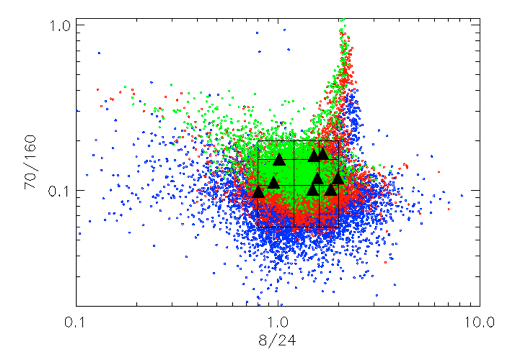
\includegraphics[width = 8 cm]{./colormaps.png}
\caption{8 - 24/70 - 160 $\mu$m colour-colour diagram of M31 obtained from IRAC and MIPS. The plot is divided into 9 regions (black grid) and the observations were made to cover those regions. The triangles indicate the regions we observed. ({\bf Needs a better explanation} )}
%\end{center}
\label{colourmaps}
\end{figure}

We obtained mid-infrared spectral maps of 12 regions in M31 using the {\em Spitzer}/IRS instrument \citep{IRS2004} covering wavelengths from 5 to 21 microns. These regions include the nucleus, two regions previously observed by ISOCAM, and 9 other regions chosen to cover a range of UV intensities, metallicities and dust temperatures. Dust temperatures were determined using a 8 - 24/70 - 160 $\mu$m colour-colour diagram (see Fig \ref{colourmaps}) which is an indicator of dust temperature. The locations of these regions are shown in Figure \ref{m31}, and their coordinates are given in Table \ref{regions}. The two regions previously observed by ISOCAM are the region from the bulge and the region from the active region in the star-forming ring (Region 9 in our sample). A background observation was also made off the galaxy along the minor axis and it was used to enable the background subtraction from the data cubes.


\begin{table}
 \centering
 \begin{minipage}{70mm}
\caption{IRS Targets and their metalicities in M31\label{regions}}
  \begin{tabular}{lccc}
  \hline Name & R.A. & Decl. &12+log(O/H)
   \\
 \hline
 Nucleus$^a$&0:42:44.31&41:16:09.4& - - -\\
Bulge$^a$&0:42:35.00&41:21:01.0&8.90$\pm$0.03\\
Region 1&0:41:30.41&40:43:07.8&9.20$\pm$0.20\\
Region 2&0:45:22.85&41:38:53.1&9.07$\pm$0.02\\
Region 3&0:40:37:37&41:01:29.4&8.85$\pm$0.01\\
Region 4&0:41:17.86&41:07:09.8&8.89$\pm$0.06\\
Region 5&0:43:39.57&41:19:03.1&\hspace{0.14cm}8.93$\pm$0.08$^b$\\
Region 6&0:43:35.72&41:23:15.0&8.73$\pm$0.08\\
Region 7&0:40:53.98&40:58:58.9&8.40$\pm$0.08\\
Region 8&0:42:21.60&41:07:17.4&\hspace{0.14cm}8.94$\pm$0.08$^b$\\
Region 9$^a$&0:41:00.00&40:36:20.3&8.86$\pm$0.02\\
NGC206&0:40:20.20&40:44:54.0& - - -\\
Background&00:44:41.8&40:58:56.0& - - -\\
\hline
\end{tabular}
{$^a$ Regions that have ISOCAM data. $^b$ Metallicity values obtained from the radial metallicity profile of M31.}
\end{minipage}
\end{table}



\begin{figure*}

\centering
%\begin{center}
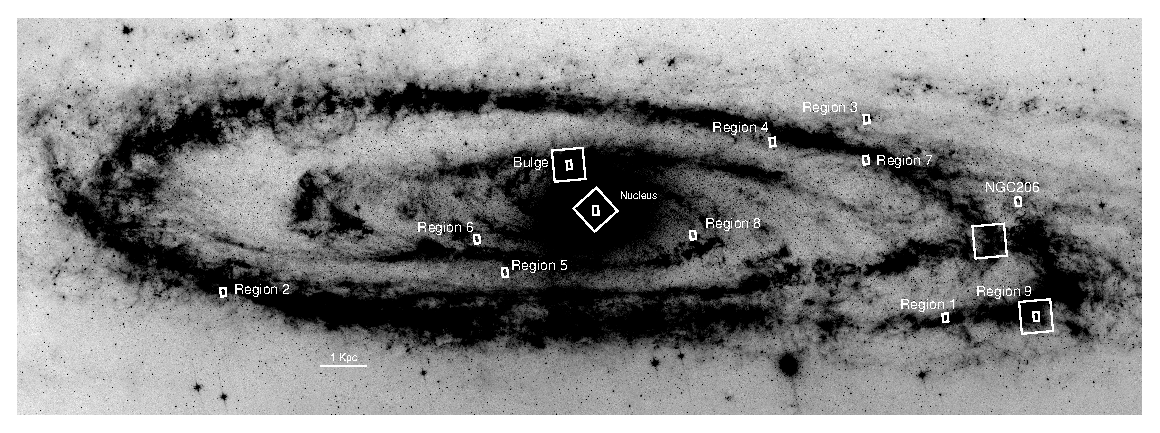
\includegraphics[scale=0.9]{./m31_map.eps}
\caption{An 8 micron IRAC image of M31 \citep{Barmby2006lr}. Small white rectangles ($30\arcsec\times50\arcsec$) show the regions that we observed and big squares ($192\arcsec\times192\arcsec$) show the regions observed by \citet{1998Cesarsky}.}
%\end{center}
\label{m31}
\end{figure*}


For our observations we used the Short-Low (SL) and Long-Low (LL) modules which cover wavelengths from 5 to 21 microns. The Low modules have a low resolving power changing from 60 - 130. Each low-resolution module is divided into two sub-slits which provide spectroscopy in either first order or second order. They are named as SL1 (7.5-14.5 $\mu$m), SL2 (5.2-7.6 $\mu$m) and LL1 (20.5-38.5 $\mu$m), LL2 (14.5-20.75 $\mu$m).

All regions were observed in September 2007 (PID 40032) with both orders of the Short-Low module (SL2, SL1) and the Long-Low order LL2. The Long-Low order LL1 was not used for observations because this spectral region contains few features. The map size was based on the size of the IRS slits (SL - $3.6\arcsec \times 57\arcsec$, LL - $10.5\arcsec \times 168\arcsec$). Each region was covered by 18 overlaping observations of the SL slit and 11 overlapping observations of the LL slit making the map size $32\arcsec \times 57\arcsec$ for SL and $58\arcsec \times 168\arcsec$ for LL. Overlapping Figure \ref{slits} shows an example of the slit arrangement. For the brighter regions (nucleus, bulge), ramp times of 14 s (SL) and 30 s (LL) were used, while for the fainter regions, ramp times of 60 and 120 s were used respectively. Background observations were taken with each module (2 per ramp time). Since all of the targets are in the same part of the sky a common background observation was used for multiple targets to subtract the background emission. 


\begin{figure}
\centering
%\begin{center}
\includegraphics[scale=0.3]{./cubeslits.eps}
\caption{SL1 data cube from the nucleus showing the arrangement of slits that has been used to cover the region. Black boxes outline the footprints of the SL1 and the green box outlines the LL2. Blue and red slits show how the each mode was covered using overlapping slit positions.}
%\end{center}
\label{slits}
\end{figure}

\subsection{IRS Data Reduction}

The data were reduced through the SSC pipeline (ver. S17.2.0) and the maps were assembled using the CUBISM program \citep{Smith:2007fk}. Bad pixel removal was also done using CUBISM and the background observations were used to subtract the background emission from these CUBES following the method outlined in \citet{Gordon:2008lr}. Spectra were extracted using a $30\arcsec\times50\arcsec$   rectangular aperture. The aperture size was selected to cover the whole overlapping area of the SL and LL modes.

After the spectral extraction there was a noticeable mismatch between the spectra from the SL1 and LL2 modules. To combine all spectra to obtain one spectrum, first a photometric comparison was conducted between the IRS spectra and the IRAC 8 micron image of M31 \citep{Barmby2006lr}. For more details about this method see the IRAC Instrument Handbook Section 4. An aperture with the same size was used to extract flux from the same regions in the IRAC 8 micron image. The photometric calibration of the IRAC is tied to point sources measured within a standard aperture with a radius of 12\arcsec. For extended sources,  an aperture correction has to be conducted as mentioned in the IRAC instrument handbook. Therefore an extended source aperture correction of 0.824 was applied for all the extractions from the 8 $\mu$m image. The uncertainty value of the IRAC image was estimated by taking the standard deviation of pixels values within an aperture of the same size from an off position of the M31 (0:48:58.00 and +42:14:54.00).

Then we stitched the SL1 and SL2 using the overlapping regions and applied a colour correction factor $K$, which is a multiplicative factor that converts the intensity of an IRS spectrum at a given wavelength to the intensity of an IRAC image taken at the same wavelength. We used the IDL code provided by the instrument handbook to compute these $K$ values for all the regions. colour correction values and the corresponding IRS data along with the IRAC data are given in Table 2.


\begin{table}
 \centering
 \begin{minipage}{90mm}
\caption{Matched aperture photometry}
  \begin{tabular}{lcccc}
  \hline{Name}&{IRS Intensity}&{IRAC Intensity}&{colour K$^b$}&{x$^{a,}$ $^c$} \\ {}&{at 8 $\mu$m$^a$}&{at 8 $\mu$m$^a$}&{}&{} 
   \\
 \hline

 Region 1 & 1.8505 & 1.3923 & 0.532 & 0.3061
 \\ Region 2  & 1.8238 & 1.3731 & 0.555 & 0.2148
 \\ Region 3 & 0.7192 & 0.9689 & 0.767 & 0.3218
 \\ Region 4 & 1.1431 & 0.8513 & 0.589 & 0.0407
 \\  Region 5 & 0.6787 & 0.8088 & 0.773 & 0.1834
 \\  Region 6  & 0.6399 & 0.7656 & 0.927 & 0.0479
 \\  Region 7  & 1.1538 & 0.8243 & 0.526 & 0.1380
 \\ Region 8 & 0.5556 & 0.7135 & 0.877 & 0.1148
 \\  Region 9 & 1.9413 & 1.6562 & 0.606 & 0.3107 
 \\ Bulge & 2.6956 & 2.5473 & 0.532 & 1.2425\\

\hline
 \label{colourK}

\end{tabular}\\
 {$^a$ Units are MJy/ sr. $^b$ colour correction factors. $^c$ Offset between IRAC and IRS as mentioned in eq. 1. Intensities are given prior to the extended source correction and the colour correction.}
\end{minipage}
\end{table}


Figure \ref{offset} compares the IRS and IRAC 8 $\mu$m photometry. The line of best fit wighted by the uncertainties has a slope of 0.81$\pm$0.08 and intercept of -0.05$\pm$0.06.  Since the intercept in Figure \ref{offset} is not zero with a higher uncertainty, it can be concluded that the offsets between orders are due to an additive offset than a multiplicative offset. Also an additive offset favours more for stitching SL and LL modes. Based on this argument, first we shifted the combined SL1 and SL2 spectrum so that the intensity at 8 $\mu$m matches with that of IRAC 8 micron image. To do this shift, the following equation was used to find the offset values (\emph{x}) between IRS and IRAC image intensities at 8 microns. 
	
\begin{equation}
F_{IRAC8} = [ F_{IRS8} + x ] \times K
%K is the colour correction factor.
\end{equation}
\footnotesize
%\emph{Where K is the colour correction factor, Flux$_{IRAC8}$ is the flux of the IRAC 8 $\mu$m image, Flux$_{IRS8}$ is the flux of IRS spectra at 8 $\mu$m and x is the offset.}
\normalsize

	
	{\em K} is the colour correction factor, F$_{IRAC8}$ is the intensity of the IRAC 8 $\mu$m image (aperture corrected) and F$_{IRS8}$ is the intensity of IRS spectra at 8 $\mu$m. The offsets for all the regions are listed in Table \ref{colourK}. After that the LL2 mode was stitched by shifting it towards the SL1 by an amount of the average difference in their overlapping spectral regions.	
	
	
\begin{figure}
\centering
%\begin{center}
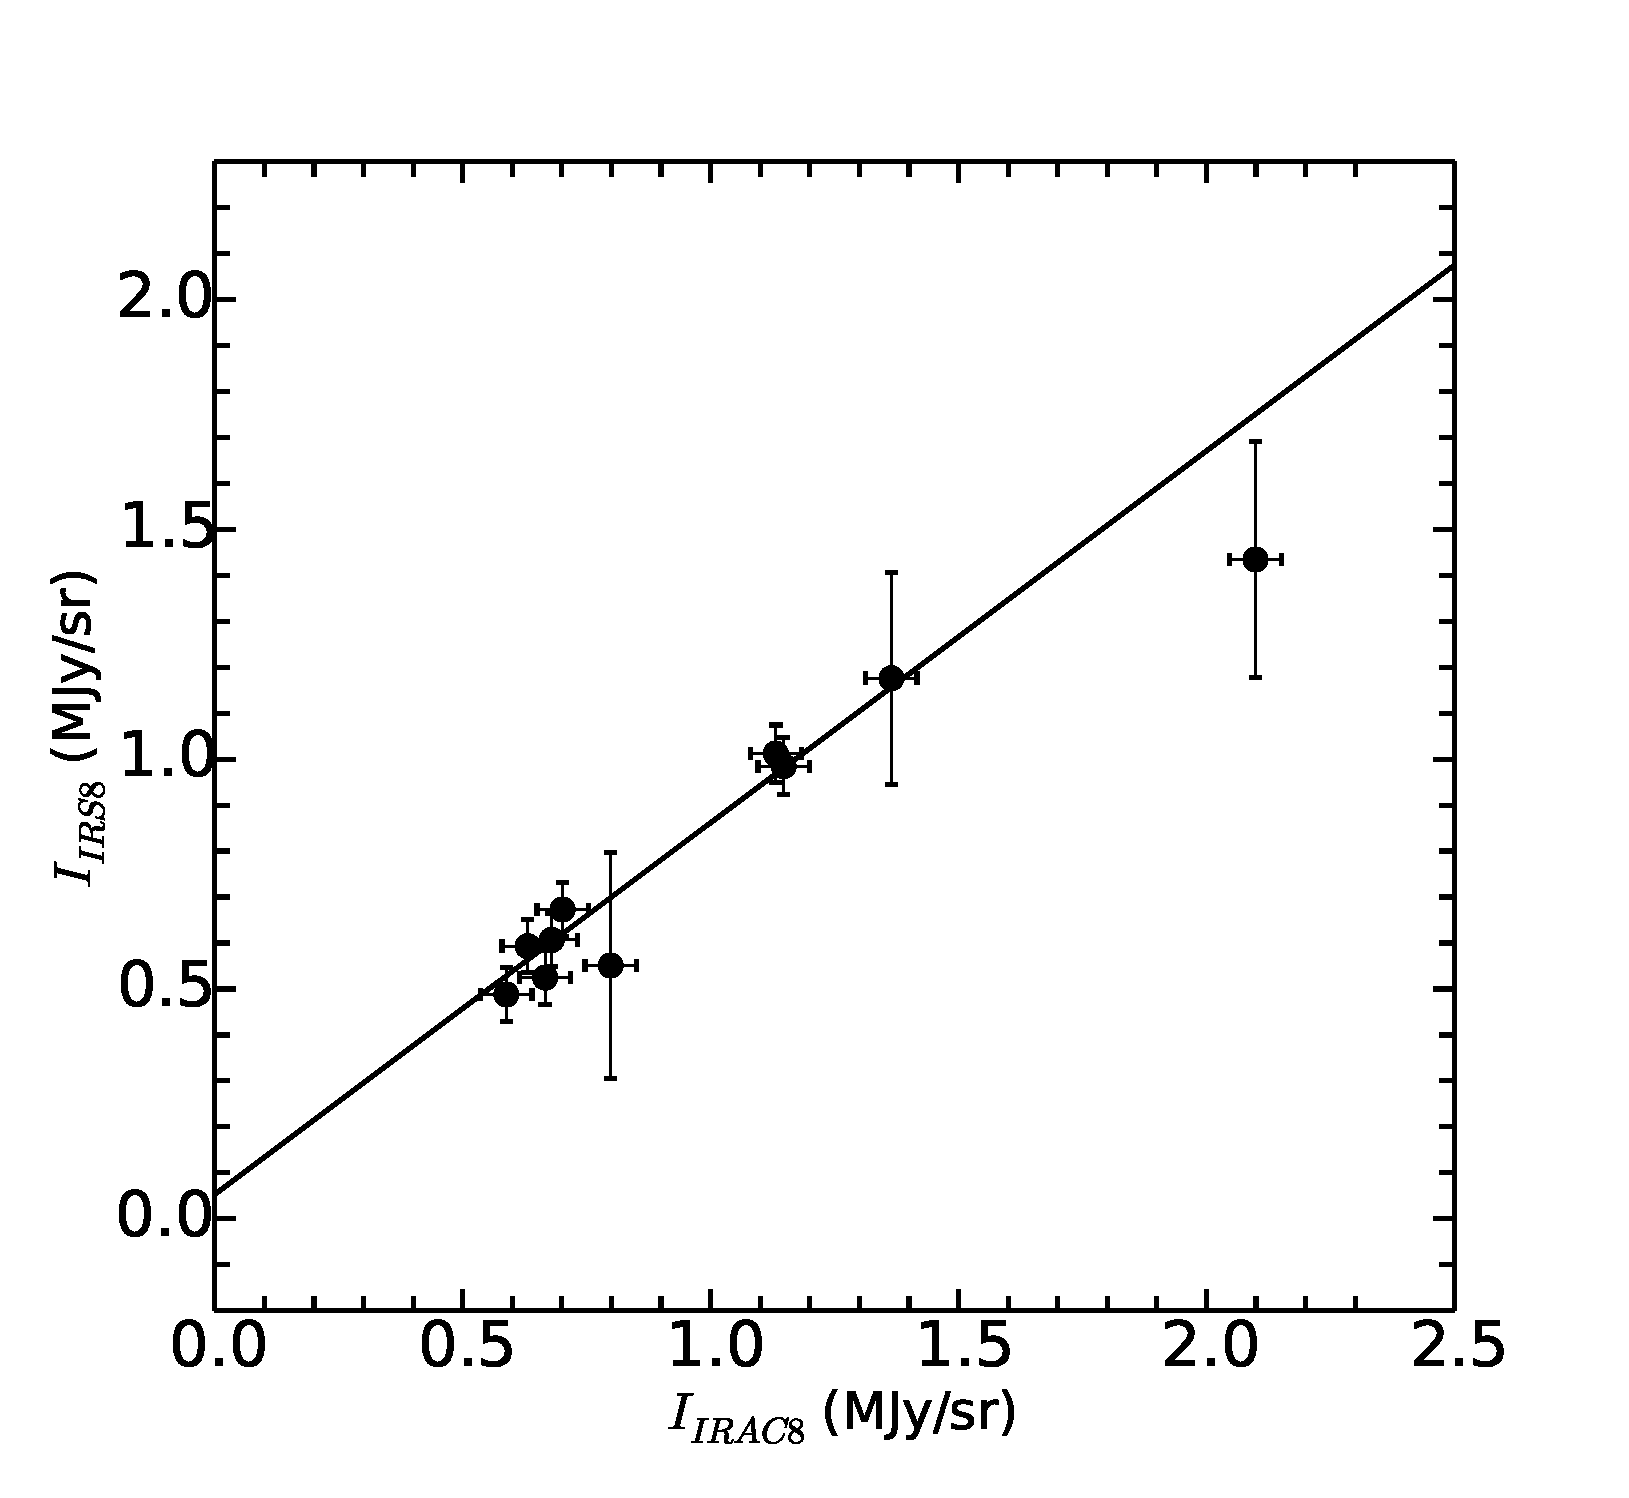
\includegraphics[scale=0.25]{./offset.eps}
\caption{ Intensity of the aperture corrected IRAC 8 $\mu$m image vs that of the colour corrected IRS spectra at 8 $\mu$m  obtained using the same aperture for our regions in M31. The straight line is the line of best fit. }
%\end{center}
\label{offset}
\end{figure}



\begin{table*}
 \centering
 \begin{minipage}{200mm}
\caption{PAH Emission Line Strengths$^a$}
  \begin{tabular}{l c c  c  c  c  c  c  c  c  c c }
  \hline {Region  }&{5.7$\mu$m  }&{6.2$\mu$m  }&{7.7$\mu$m  }&{8.3$\mu$m  }&{8.6$\mu$m  }&{10.7$\mu$m  }&{11.3$\mu$m  }&{12.0$\mu$m  }&{12.7$\mu$m  }&{17.0$\mu$m  } 
   \\
 \hline



 Region 1 &10$\pm$1            & 34$\pm$1-09        & 107$\pm$10        & 13$\pm$1       & 14.1$\pm$0.9        & 2.2$\pm$0.3        & 33.4$\pm$0.9        & 9.1$\pm$0.5        & 16$\pm$1        & 17$\pm$1        \\
Region 2 &7.7$\pm$0.9        & 31.2$\pm$0.8        & 106$\pm$8        & 9$\pm$1           & 19.8$\pm$0.8        & 1.5$\pm$0.2        & 32.0$\pm$0.8        & 6.6$\pm$0.4        & 15$\pm$1        & 14.7$\pm$0.9        \\
Region 3 &8$\pm$4              & 25$\pm$3                & 111$\pm$22       & 21$\pm$4       & 7$\pm$3                 & 1.1$\pm$0.9        & 19$\pm$3             & 6$\pm$1             & 14$\pm$3           & 13$\pm$2        \\
Region 4 &4$\pm$1              & 15.8$\pm$0.9        & 59$\pm$9        & 7$\pm$1           & 11.6$\pm$0.8          & 0.8$\pm$0.2        & 19.9$\pm$0.8        & 3.5$\pm$0.4        & 9$\pm$1             & 12.5$\pm$0.9        \\
Region 5 &1$\pm$1              & 7$\pm$1                 & 22$\pm$3        & 3$\pm$1           & 5.8$\pm$0.8            & 0.9$\pm$0.2        & 12.7$\pm$0.8        & 2.4$\pm$0.4        & 6.3$\pm$0.4        & 10$\pm$2        \\
Region 6 & - - - -                      & 7.3$\pm$0.9         & 22$\pm$7        & 3$\pm$1            & 3.6$\pm$0.8            & 0.8$\pm$0.2        & 10.8$\pm$0.8        & 1.9$\pm$0.4        & 4.5$\pm$0.4        & 8.3$\pm$0.6        \\
Region 7 &5.9$\pm$0.9        & 17.7$\pm$0.9       & 57$\pm$8        & 9$\pm$1            & 12.8$\pm$0.8        & 1.6$\pm$0.2        & 21.8$\pm$0.8        & 5.2$\pm$0.4        & 11$\pm$1             & 13$\pm$2        \\
Region 8 &2.$\pm$1              & 3$\pm$1              & 6$\pm$3            & 3$\pm$1            & 2.7$\pm$0.8        & 1.4$\pm$0.3        & 4.4$\pm$0.8            & - - - -                      &  - - - -                       & 4.1$\pm$0.7        \\
Region 9 &  - - - -                     & 38$\pm$3          & 133$\pm$29        & 25$\pm$4        & 15$\pm$3            & 2.4$\pm$0.8        & 37$\pm$3               & 14$\pm$1             & 25$\pm$3        & 19$\pm$6        \\
Bulge       & - - - -                       & 38$\pm$2           & 219$\pm$27        & 32$\pm$4        & 20$\pm$3           & 2.0$\pm$0.9        & 53$\pm$3              & 14$\pm$1           & 29$\pm$3        & 39$\pm$2       \\

\hline
 \label{PAHlinetable}
\end{tabular}\\
{$^a$ Units are 10$^{-9}$ W/m$^2$.}
\end{minipage}
\end{table*}







\begin{table*}
 \centering
 \begin{minipage}{200mm}
\caption{PAH Emission Line Equivalent Widths$^a$}
  \begin{tabular}{l c c  c  c  c  c  c  c  c  c c }
  \hline {Name  }&{5.7$\mu$m  }&{6.2$\mu$m  }&{7.7$\mu$m  }&{8.3$\mu$m  }&{8.6$\mu$m  }&{10.7$\mu$m  }&{11.3$\mu$m  }&{12.0$\mu$m  }&{12.7$\mu$m  }&{17.0$\mu$m  } 
   \\
 \hline



 Region 1 &0.39$\pm$0.08        & 1.2$\pm$0.1             & 3.4$\pm$0.3        & 0.43$\pm$0.04        & 0.47$\pm$0.04        & 0.09$\pm$0.01        & 1.45$\pm$0.04        & 0.43$\pm$0.03        & 0.78$\pm$0.03              & 1.27$\pm$0.05        \\
 Region 2 &0.28$\pm$0.04        & 1.02$\pm$0.06        & 3.4$\pm$0.2        & 0.32$\pm$0.04        & 0.70$\pm$0.04        & 0.07$\pm$0.01        & 1.58$\pm$0.04        & 0.35$\pm$0.02        & 0.85$\pm$0.03              & 1.35$\pm$0.06        \\
 Region 3$^b$ &4$\pm$2           & 8$\pm$2                   & 19$\pm$4            & 2.8$\pm$0.8             & 0.9$\pm$0.5             & 0.1$\pm$0.1            & 2.1$\pm$0.3             & 0.7$\pm$0.2            & 1.6$\pm$0.2                   & 2.4$\pm$0.3        \\
 Region 4 &0.28$\pm$0.09        & 1.0$\pm$0.1             & 3.7$\pm$0.4       & 0.5$\pm$0.1              & 0.77$\pm$0.07        & 0.07$\pm$0.02        & 1.67$\pm$0.06        & 0.31$\pm$0.04        & 0.86$\pm$0.05             & 1.68$\pm$0.07        \\
 Region 5 & - - - -        & 0.12$\pm$0.03        & 0.61$\pm$0.08   & 0.10$\pm$0.03        & 0.20$\pm$0.03        & 0.05$\pm$0.01        & 0.77$\pm$0.03        & 0.17$\pm$0.03        & 0.50$\pm$0.04            & 1.6$\pm$0.2        \\
 Region 6 & - - - -                          & 0.10$\pm$0.04        & 0.6$\pm$0.2        & 0.10$\pm$0.04        & 0.14$\pm$0.03        & 0.05$\pm$0.01        & 0.77$\pm$0.04        & 0.15$\pm$0.03        & 0.42$\pm$0.04            & 1.7$\pm$0.1        \\
 Region 7 &0.32$\pm$0.05        & 0.86$\pm$0.06        & 2.8$\pm$0.2        & 0.44$\pm$0.06        & 0.69$\pm$0.06        & 0.12$\pm$0.02        & 1.81$\pm$0.07        & 0.48$\pm$0.05        & 1.11$\pm$0.08            & 2.2$\pm$0.2        \\
 Region 8 &0.03$\pm$0.04        & 0.04$\pm$0.03        & 0.2$\pm$0.10      & 0.09$\pm$0.04        & 0.10$\pm$0.03        & 0.09$\pm$0.02        & 0.30$\pm$0.02        & 0.00$\pm$0.00        & 0.01$\pm$0.01            & 0.62$\pm$0.07        \\
 Region 9$^b$ & - - - -                 & 237$\pm$100          & 151$\pm$60        & 16$\pm$6                 & 8$\pm$3                   & 0.5$\pm$0.2             & 7$\pm$1                   & 2.3$\pm$0.6             & 3.6$\pm$0.8                 & 2.4$\pm$0.8  \\
 Bulge       & - - - -                          & 1.2$\pm$0.2            & 4.0$\pm$0.4        & 0.51$\pm$0.07         & 0.30$\pm$0.06        & 0.03$\pm$0.01        & 0.78$\pm$0.03        & 0.22$\pm$0.02        & 0.49$\pm$0.03            & 1.16$\pm$0.04 \\       


\hline
 \label{EQW}
\end{tabular}\\
{$^a$ Units are $\mu$m. $^b$ EQWs from these two regions were removed from the analysis (see section 3.2).}
\end{minipage}
\end{table*}






\begin{table*}
 \centering
 \begin{minipage}{100mm}
\caption{Atomic Emission Line Strengths$^a$}
  \begin{tabular}{l c c  c  c  c  c  }
  \hline{Name  }&{[Ar~{\sc ii}] }&{[Ar~{\sc iii}]  }&{[S~{\sc iv}]}&{[Ne~{\sc ii}]   }&{[Ne~{\sc iii}]   }&{[S~{\sc iii}]  }\\
{}&{\tiny{7.0$\mu$m} }&{\tiny{9.0$\mu$m }}&{\tiny{10.5$\mu$m}}&{\tiny{12.8$\mu$m  }}&{\tiny{15.5$\mu$m } }&{\tiny{18.7$\mu$m }} 
   \\
 \hline 
 
Region 1 &    $<$15.2                 & $<$16.4                 & 6$\pm$1                 & 6$\pm$1                 & $<$ 4.2                 & 2.2$\pm$0.4                \\
Region 2 &    5$\pm$3                 & $<$ 17.4               & $<$5.1                    & 6$\pm$1                 & $<$ 2.9                 & 0.9$\pm$0.5                 \\
Region 3 &    $<$42.9                 & 27$\pm$6              & $<$ 28.9                & 9$\pm$3                 & 6$\pm$1               & 4.3$\pm$0.9                 \\
Region 4 &    $<$11.2                 & $<$10.0                 & $<$4.4                    & 2$\pm$1                 & 0.6$\pm$0.5        & 1.3$\pm$0.5                 \\
Region 5 &    4$\pm$3                 & $<$6.2                   & $<$ 5.2                 & $<$ 4.2                     & 2$\pm$1               & 2$\pm$1                 \\
Region 6 &    7$\pm$3                & 4$\pm$2                 & $<$ 3.8                 & 2$\pm$1                  & 5.4$\pm$0.5         & 5.3$\pm$0.5                 \\
Region 7 &    3$\pm$3                 & $<$12.6                 & 2.3$\pm$0.9        & 10$\pm$2                & $<$ 2.9                 & 8$\pm$1                \\
Region 8 &    $<$11.8                  & 5$\pm$2                & $<$4.9                  & $<$2.6                       & 11.6$\pm$0.5     & 6.5$\pm$0.5                 \\
Region 9 &    24$\pm$10             & 35$\pm$8             & $<$ 2.7                 & 38$\pm$3                 & 7$\pm$4               & 15.3$\pm$5.6                 \\
Bulge &          10$\pm$7               & 49$\pm$7              & $<$ 30.4               & 19$\pm$4                 & 7$\pm$2               & 2$\pm$1      \\           

\hline
 \label{Atomic}
\end{tabular}\\
{ $^a$ Units are 10$^{-10}$ W/m$^2$. Upper limits are indicated with a $<$ mark.  }
\end{minipage}
\end{table*}



\subsection{ISOCAM Data Reduction}


To compare our results with previous observations, ISOCAM data of three regions previously observed by \citet{1998Cesarsky} which overlap with IRS observations were obtained. We retrieved the highly processed data provided by \citet{Boulanger_F_2005} of these ISOCAM observations. The total wavelength range covered was 5.15 to 16.5 $\mu$m and the field-of-view was 32$\times $32 pixels with 6\arcsec\ per pixel. An image of the ISOCAM data is shown in Figure \ref{isonuc}.  For the three regions in common, we extracted spectra using the same aperture as for the IRS data. 


\begin{figure}
\centering
%\begin{center}
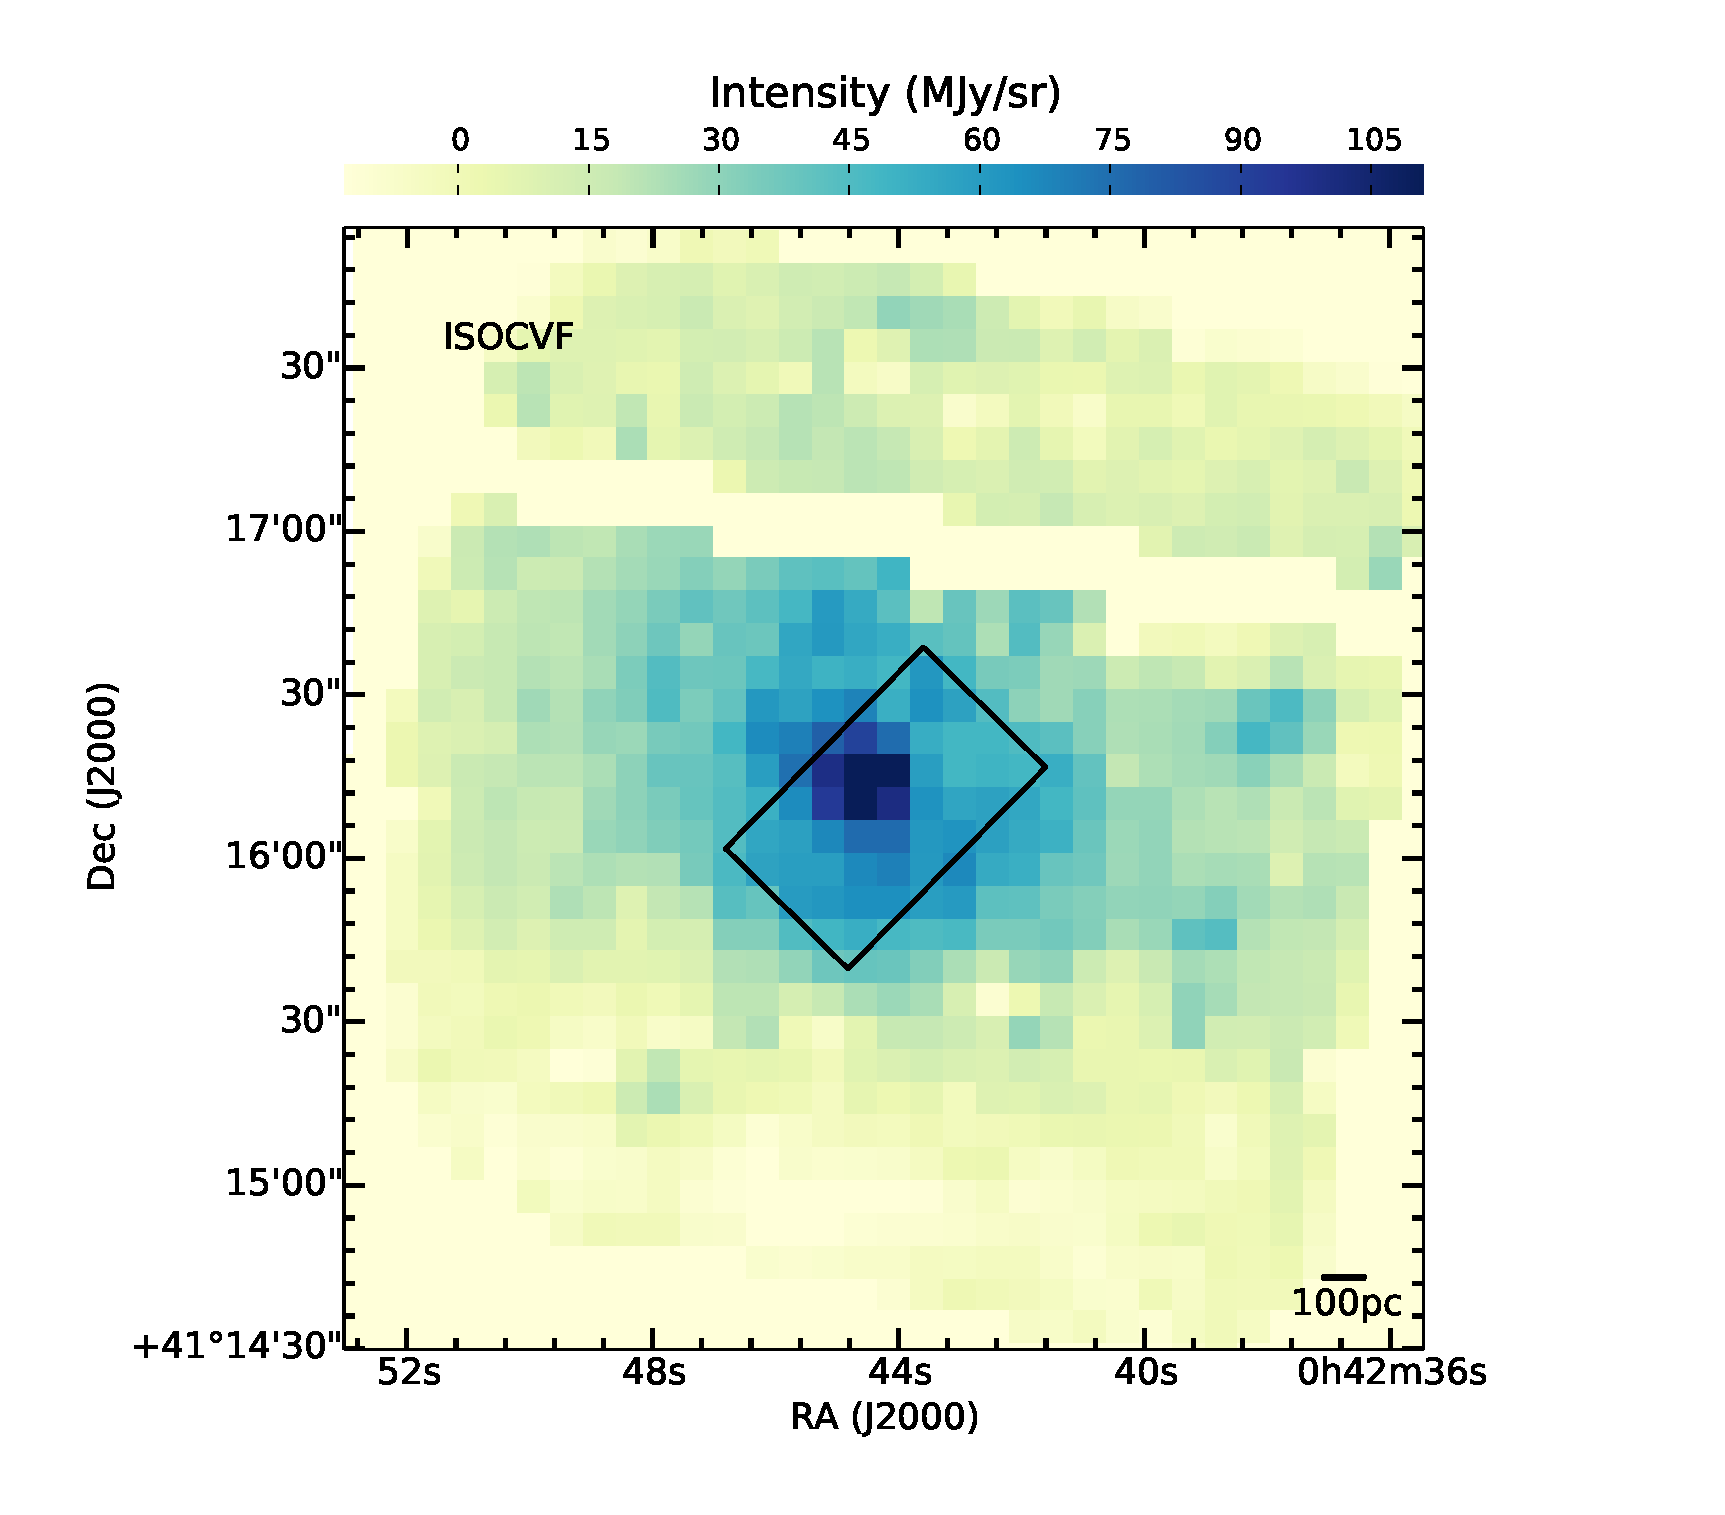
\includegraphics[width = 8cm]{./isonuc.eps}
\caption{11.3 $\mu$m image of the ISOCAM data cube from the nucleus of M31. The black box shows the size of the aperture that used to extract spectra.}
%\end{center}
\label{isonuc}
\end{figure}

\section{Data Analysis}

All the main PAH features features, including the 6.2, 7.7, 8.6 and 11.3 $\mu$m bands, are clearly visible in the final processed spectra (see Figures \ref{PAHFITplots}) from all the regions except the nucleus (The spectrum of the nucleus is discussed in Section 4.3). They also show atomic line emissions such as [Ar~{\sc ii}], [Ar~{\sc iii}], [S~{\sc iii}], [S~{\sc iv}], [Ne~{\sc ii}], [Ne~{\sc iii}] and molecular $H_{2}$ emission at 12.3 $\mu$m. Some of the spectra display a contribution to the continuum from starlight emission.

Dust continuum emission from the Regions 3 and 9 is very low compared to other spectra and they also show some negative flux values in the shorter wavelengths which can be due to instrumental errors. It was observed that the spectrum from the NGC 206 is very noisy, therefore that spectrum was removed from our analysis. 


\subsection{ISOCAM versus IRS }


As mentioned in the Introduction, based on ISOCAM observations \citet{1998Cesarsky} reported a suppression of the common 6 to 8 $\mu$m features and an enhancement of a broad 11.3 and 12.7 $\mu$m features in four regions of M31. In addition, \citet{Pagani_1999} confirmed that the star-forming ring in M31 shows very weak PAH emission in the 6 to 8 $\mu$m region. 
However, the IRS spectra presented here do not show such unusual behaviour (Figure \ref{PAHFITplots}). Indeed, except for the nucleus, all regions show a normal mid-IR spectrum similar to other nearby starforming galaxies. Therefore, we obtained newly-processed ISOCAM spectra from three regions in our IRS sample (see Section 2.4) and compare them with the corresponding IRS spectra (Figure \ref{ISOnIRS}). 

	The spectra from both instruments look almost the same. Although the relative intensity of the features in the IRS and ISOCAM spectra are differ in detail, the shapes of the spectra are almost identical. Except for the nucleus, there is no depletion in 6 to 8 $\mu$m features as described in \citet{1998Cesarsky}. 
	
	Until 2005, ISOCAM data were not properly background subtracted and they were contaminated with zodiacal emission and stray light. Therefore, differential spectra between regions of relatively strong and weak emission have been used to overcome this problem (more details about the differential spectra can be found in \citealt{1998Cesarsky}). In 2005, the ISOCAM data were reprocessed  and corrected for the zodiacal emission \citep{Boulanger_F_2005}. For the remainder of this paper the reprocessed ISOCAM data are referred to as ISO2005 and earlier data as ISO1998. It is clear that the spectra obtained from these newly processed ISOCAM data do not agree with the previous differential spectra, especially for the bulge and the nucleus. Indeed, the differential spectrum shows a broad emission around the 11.3 micron feature not visible in Figure \ref{ISOnIRS} (top). Also, the differential spectrum towards the bulge does not show any emission in the 6 to 8 $\mu$m region unlike the newly processed data (Figure \ref{ISOnIRS} middle).

	By examining the spectra obtained from other regions (Figure 8 $\&$ 9) which were observed by IRS instrument, it can be argued that the IRS results do not support the results based on ISO1998 data.


\begin{figure}
\centering
%\begin{center}
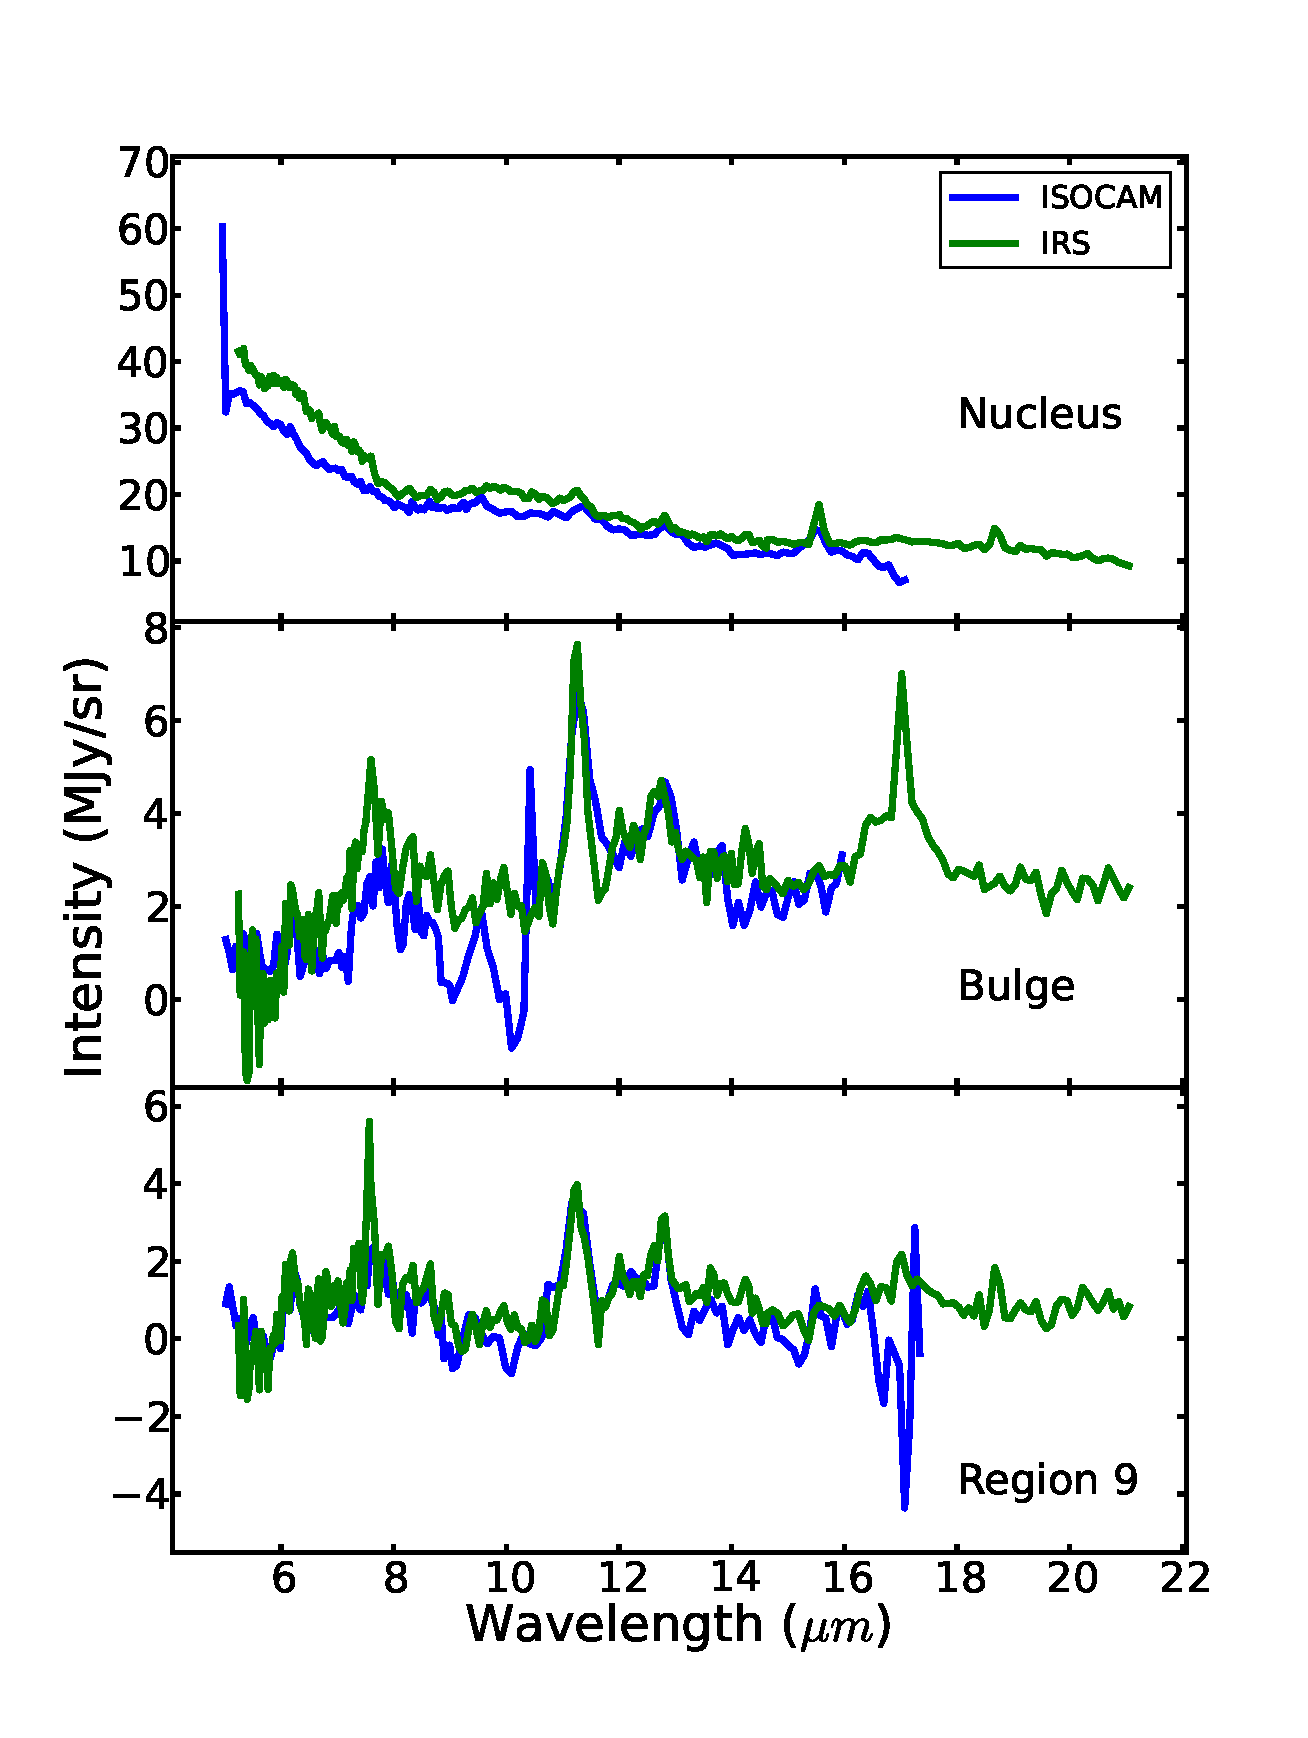
\includegraphics[scale=0.35]{./ISOvsIRS.eps}
\caption{ Comparison of the IRS and the newly processed ISOCAM spectra for the Nucleus (top), Bulge (middle) and Region 9 (bottom) in M31.}
%\end{center}
\label{ISOnIRS}
\end{figure}


\subsection{PAHFIT}

The PAH features in the IRS spectra are often blended with neighbouring aromatic features and atomic lines. Therefore measuring the strength of PAH features is difficult. To achieve this task a tool called PAHFIT, introduced by \citet{Smith:2007lr}, was used. PAHFIT is an IDL  based tool designed for decomposing {\em Spitzer} IRS spectra of PAH emission sources and is capable of identifying PAH features among other blended features. It also takes silicate absorption and extinction into account. PAHFIT is primarily designed for use with full 5-35 micron {\em Spitzer} low-resolution IRS spectra.

PAHFIT uses six main components to fit the surface brightness. These are starlight continuum, featureless thermal dust continuum, pure rotational lines of $H_2$, fine-structure lines, dust emission features and dust extinction. The starlight is represented by a modified blackbody emission at a fixed temperature of 5000 K and the dust continuum is represented by 8 modified blackbodies at fixed temperatures of 35, 40, 50, 65, 90, 135, 200, 300 K. However, the final fit obtained with PAHFIT does not necessarily take all dust continua into account. Line features are represented by Gaussian profiles and dust features are represented by Drude profiles. The infrared extinction is considered as a combination of a power law plus silicate features peaking at 9.7 and 18 $\mu$m. More details about PAHFIT can be found in \citet{Smith:2007lr}.

None of the IRS spectra shows a significant silicate absorption around 9.7 or 18 $\mu$m and the the extinction values calculated by PAHFIT were almost zero. Therefore, we adjusted the PAHFIT input parameters so that it does not take dust extinction into account. Except for the bulge, Region 5, Region 6 and Region 8, the spectra do not show much contribution from starlight. Therefore, the starlight parameter in PAHFIT was also set to zero so that it does not take starlight into account except for the regions mentioned above. 

PAHFIT did not fit the spectrum from the nucleus properly. This was due to the silicate emission around 9.7 $\mu$m and therefore we did not use PAHFIT data from the nucleus for our analysis.





\begin{figure*}
\centering
%\begin{center}
\includegraphics[scale=0.45]{./ALL.eps}
  \caption{The spectra from 10 regions (black squares) shown with their detailed PAHFIT decomposition. Red, blue, light blue, pink and green lines represent the dust continua, PAH features, atomic lines, starlight continuum and the fit respectively. The black line shows the total continuum. Spectra from the nucleus and NGC 206 is not shown here.}
\label{PAHFITplots}
\end{figure*}


\subsection{PAH Features}

PAHFIT returns fluxes and equivalent widths (EQWs) of PAH features which are given in Table \ref{PAHlinetable} and \ref{EQW}. The intensities of the features do not include any contribution from the continuum but the equivalent width computed by


\begin{equation}
EQW=\int \frac{I_{\nu} - I_{\nu(cont)}}{I_{\nu(cont)}} \,d\lambda,
\end{equation}

is a measure of both the strength of the continuum emission (\(I_{\nu(cont)} \)) and the line strength (\(I_{\nu(feature)}\)). Here \(I_{\nu} = I_{\nu(feature)} + I_{\nu(cont)}\). The continuum emission is mainly coming from the dust grains. Hence, by studying EQWs of PAHs, we can study how the PAHs compete with the dust grains in the mid-IR wavelengths. Therefore the EQW values were obtained to analyze the characteristics of PAHs in M31. PAHFIT returns the EQW values for each PAH feature and the uncertainties were calculated using a Monte-Carlo method. In that method, for each region, PAHFIT was run 500 times on randomly generated data points  normally distributed within the uncertainties of the spectrum. PAHFIT returned 500 EQW values for each PAH feature and the standard deviation of EQWs for a given feature was taken as its uncertainty. 
The EQW values from IRC3 and ISOCVF regions were removed from our analysis because they have negative flux values in their spectra which can affect the EQWs. 



\subsection{Atomic Line Features}
\begin{figure}

\centering
%\begin{center}
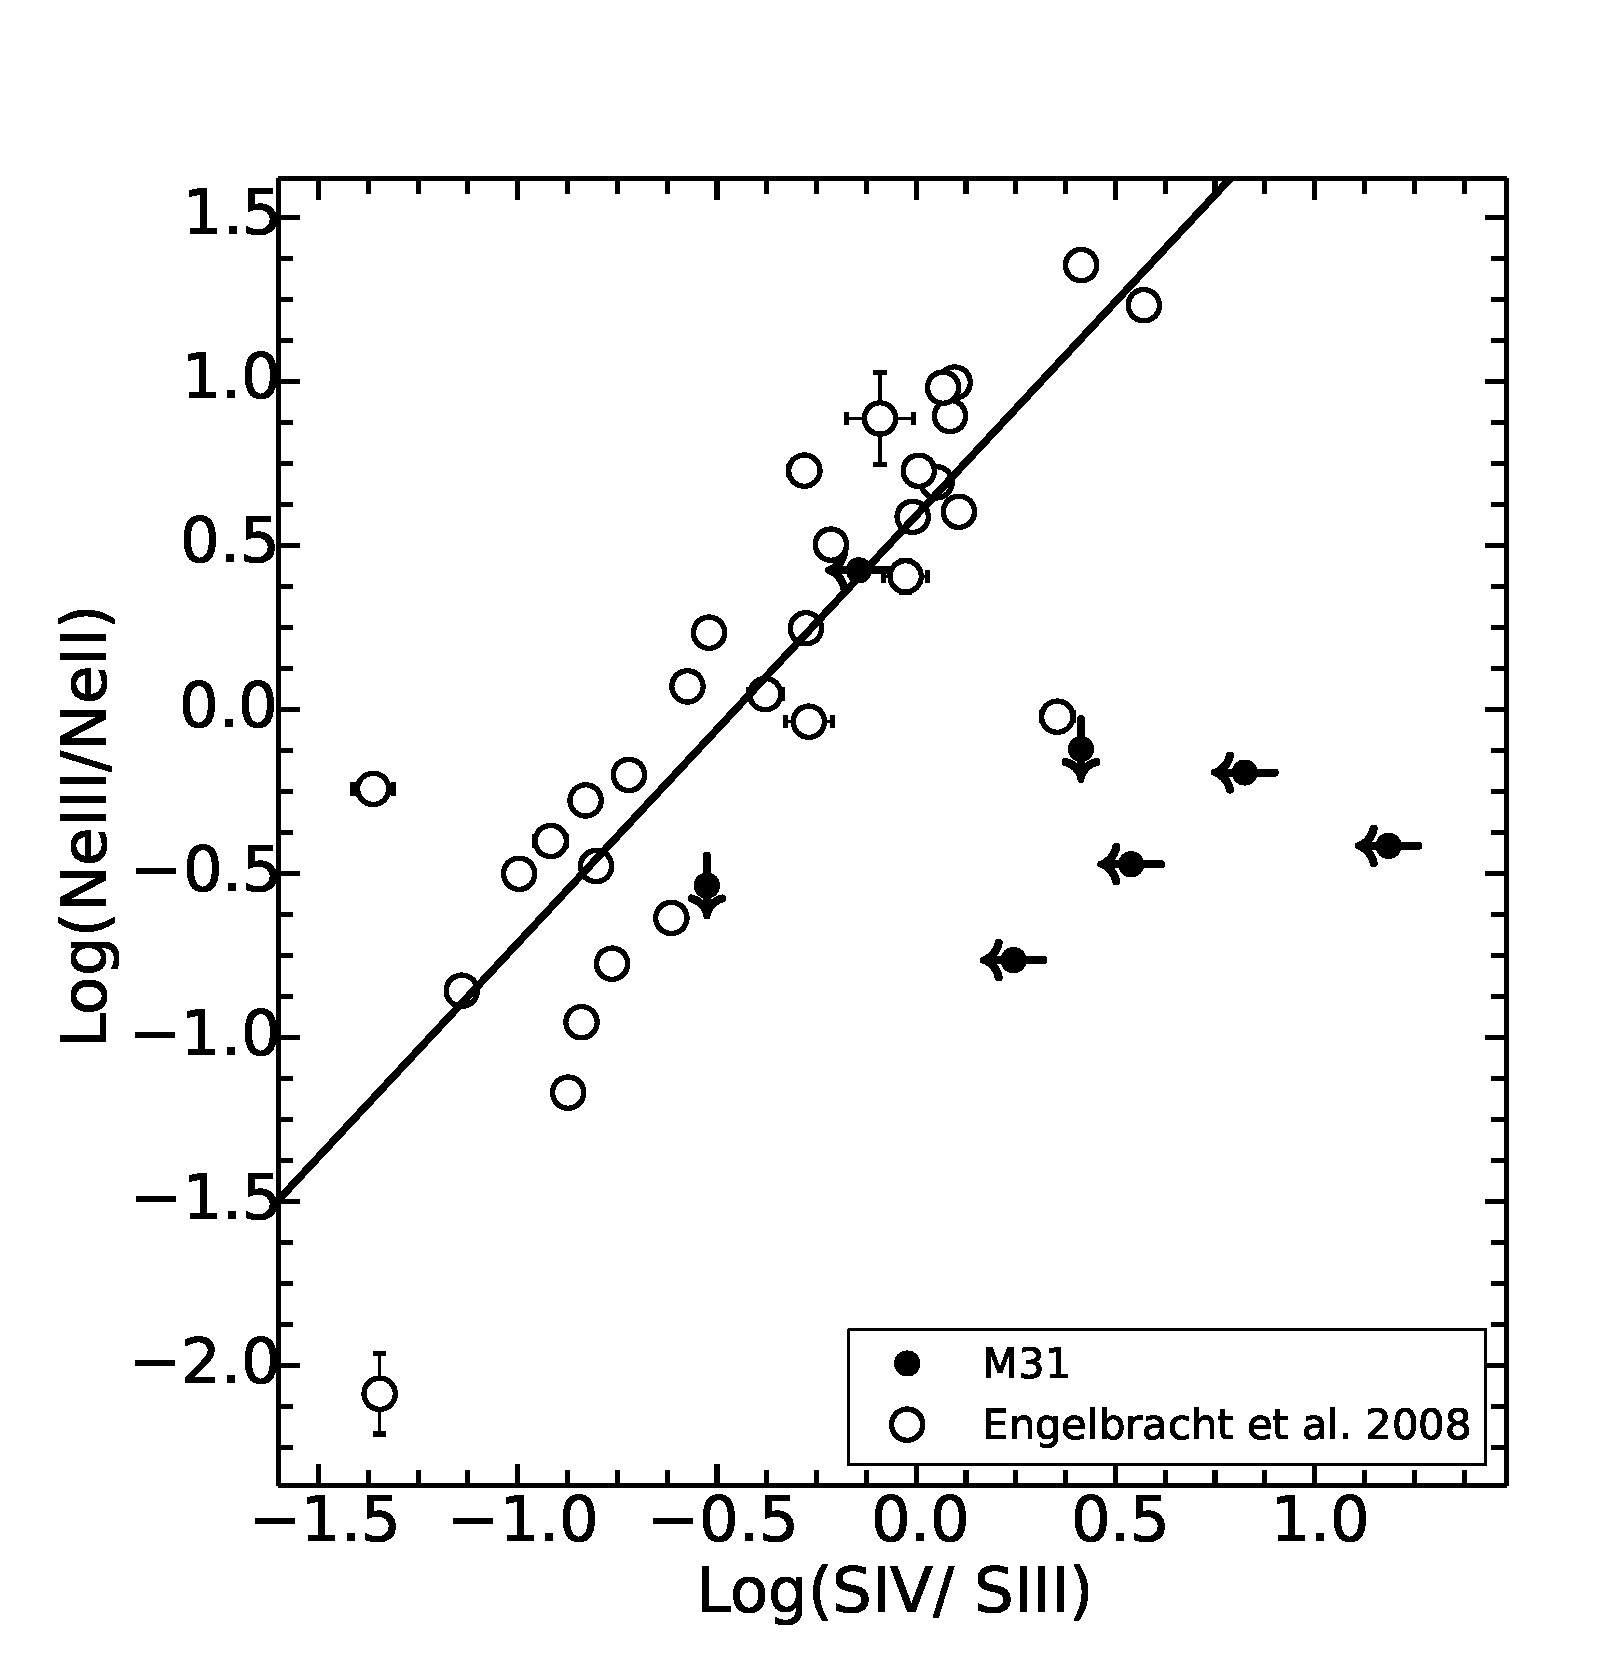
\includegraphics[scale=0.3]{./NevsS.eps}
\caption{ Log([Ne~{\sc iii}]/[Ne~{\sc ii}])  vs Log([S~{\sc iv}]/[S~{\sc iii}]) 18 for the M31 regions in our sample (black dots) and for the starburst sample from Engelbracht (2008; open dots). The straight line is the line of best fit for the starburst sample.}
%\end{center}
\label{SvsNe}
\end{figure}

PAHFIT also returns the emission line strengths and the flux uncertainties of atomic lines. These are listed in Table 4.

	Line ratios of [Ne~{\sc iii}]/[Ne~{\sc ii}] and [S~{\sc iv}]/[S~{\sc iii}] 18 have been used as an indication of the radiation hardness. \citet{Engelbracht_2008} demonstrated that a combination of these two line ratios -which they call the radiation hardness index (RHI)- is a more sensitive indicator of the hardness of the radiation. The RHI values are calculated using
\vspace{5 mm}	
\begin{equation}
{RHI = \left( \log\frac{\textrm{[Ne~{\sc iii}] }}{\textrm{[Ne~{\sc ii}]}} + [0.71 + 1.58\log\frac{\textrm{{[S~{\sc iv}]}}}{\textrm{{[S~{\sc iv}]}}}\right) /2}
\vspace{5 mm}	
\end{equation}

	Here, 1.58 and 0.71 are the slope and the intercept of the [Ne~{\sc iii}]/[Ne~{\sc ii}]  vs [S~{\sc iv}]/[S~{\sc iii}] 18 plot (Figure \ref{SvsNe}) for the starburst sample from \citet{Engelbracht_2008}. The RHI has also been used by \citet{Gordon:2008lr} for M101 observations. To investigate whether the atomic line emission from the selected regions of M31 with the fit parameters described above, we compared them to the starburst sample (Figure \ref{SvsNe}). 
	
	We calculated upper limits for non-detected lines \footnote{To find the upper limits for the flux of missing atomic lines, we assumed the line to be a Gaussian profile with a FWHM as given by PAHFIT. The peak intensity was taken to be 3 times the RMS, where RMS is the root mean square of the noise at the position of a missing line.}. Figure \ref{SvsNe}  shows that the limits are reasonably following the trend for the starburst galaxy sample. Therefore the equation mentioned above was adopted with a simple modification to calculate the RHI values for our sample. For the regions with missing Ne lines, equations 4 was used and for the regions with missing S lines, equation 5 was used. 




\vspace{2 mm}	
\begin{equation}
RHI = \left(0.71 + 1.58\log\frac{\textrm{[S~{\sc iv}]}}{\textrm{[S~{\sc iii}]}}\right)
\vspace{1 mm}	
\end{equation}

\vspace{1 mm}	
\begin{equation}
RHI = \left(\log\frac{\textrm{[Ne~{\sc iii}]}}{\textrm{[Ne~{\sc ii}]}}\right)
\vspace{5 mm}	
\end{equation}
		%\vspace{5 mm}
		
		For Region 2, Region 5 and Region 8 regions, we used the upper limit values of their atomic line intensities to calculated RHI values.
	


\section{Results and Discussion}


\subsection{PAH intensities}

Both the 6.2 and 7.7 $\mu$m features are thought to be coming from ionized PAHs and the 11.3 $\mu$m feature is from neutral PAHs. Therefore we expect to see a correlation between the intensities of 6.2 and 7.7 $\mu$m PAH features normalized by the 11.3 $\mu$m feature. In Figure \ref{PAHlines} we compared the PAH flux ratios of 7.7/11.3  and 6.2/11.3 features. The figure shows a good correlation between these two PAH line ratios and it consistent with that of SINGS sample in \citet{Smith:2007lr}. This correlation has also been reported in \citet{Galliano2008} and \citet{Vermeij2002}. This evident that the PAH emission from M31 is not unusual. 

\begin{figure}
\centering
%\begin{center}
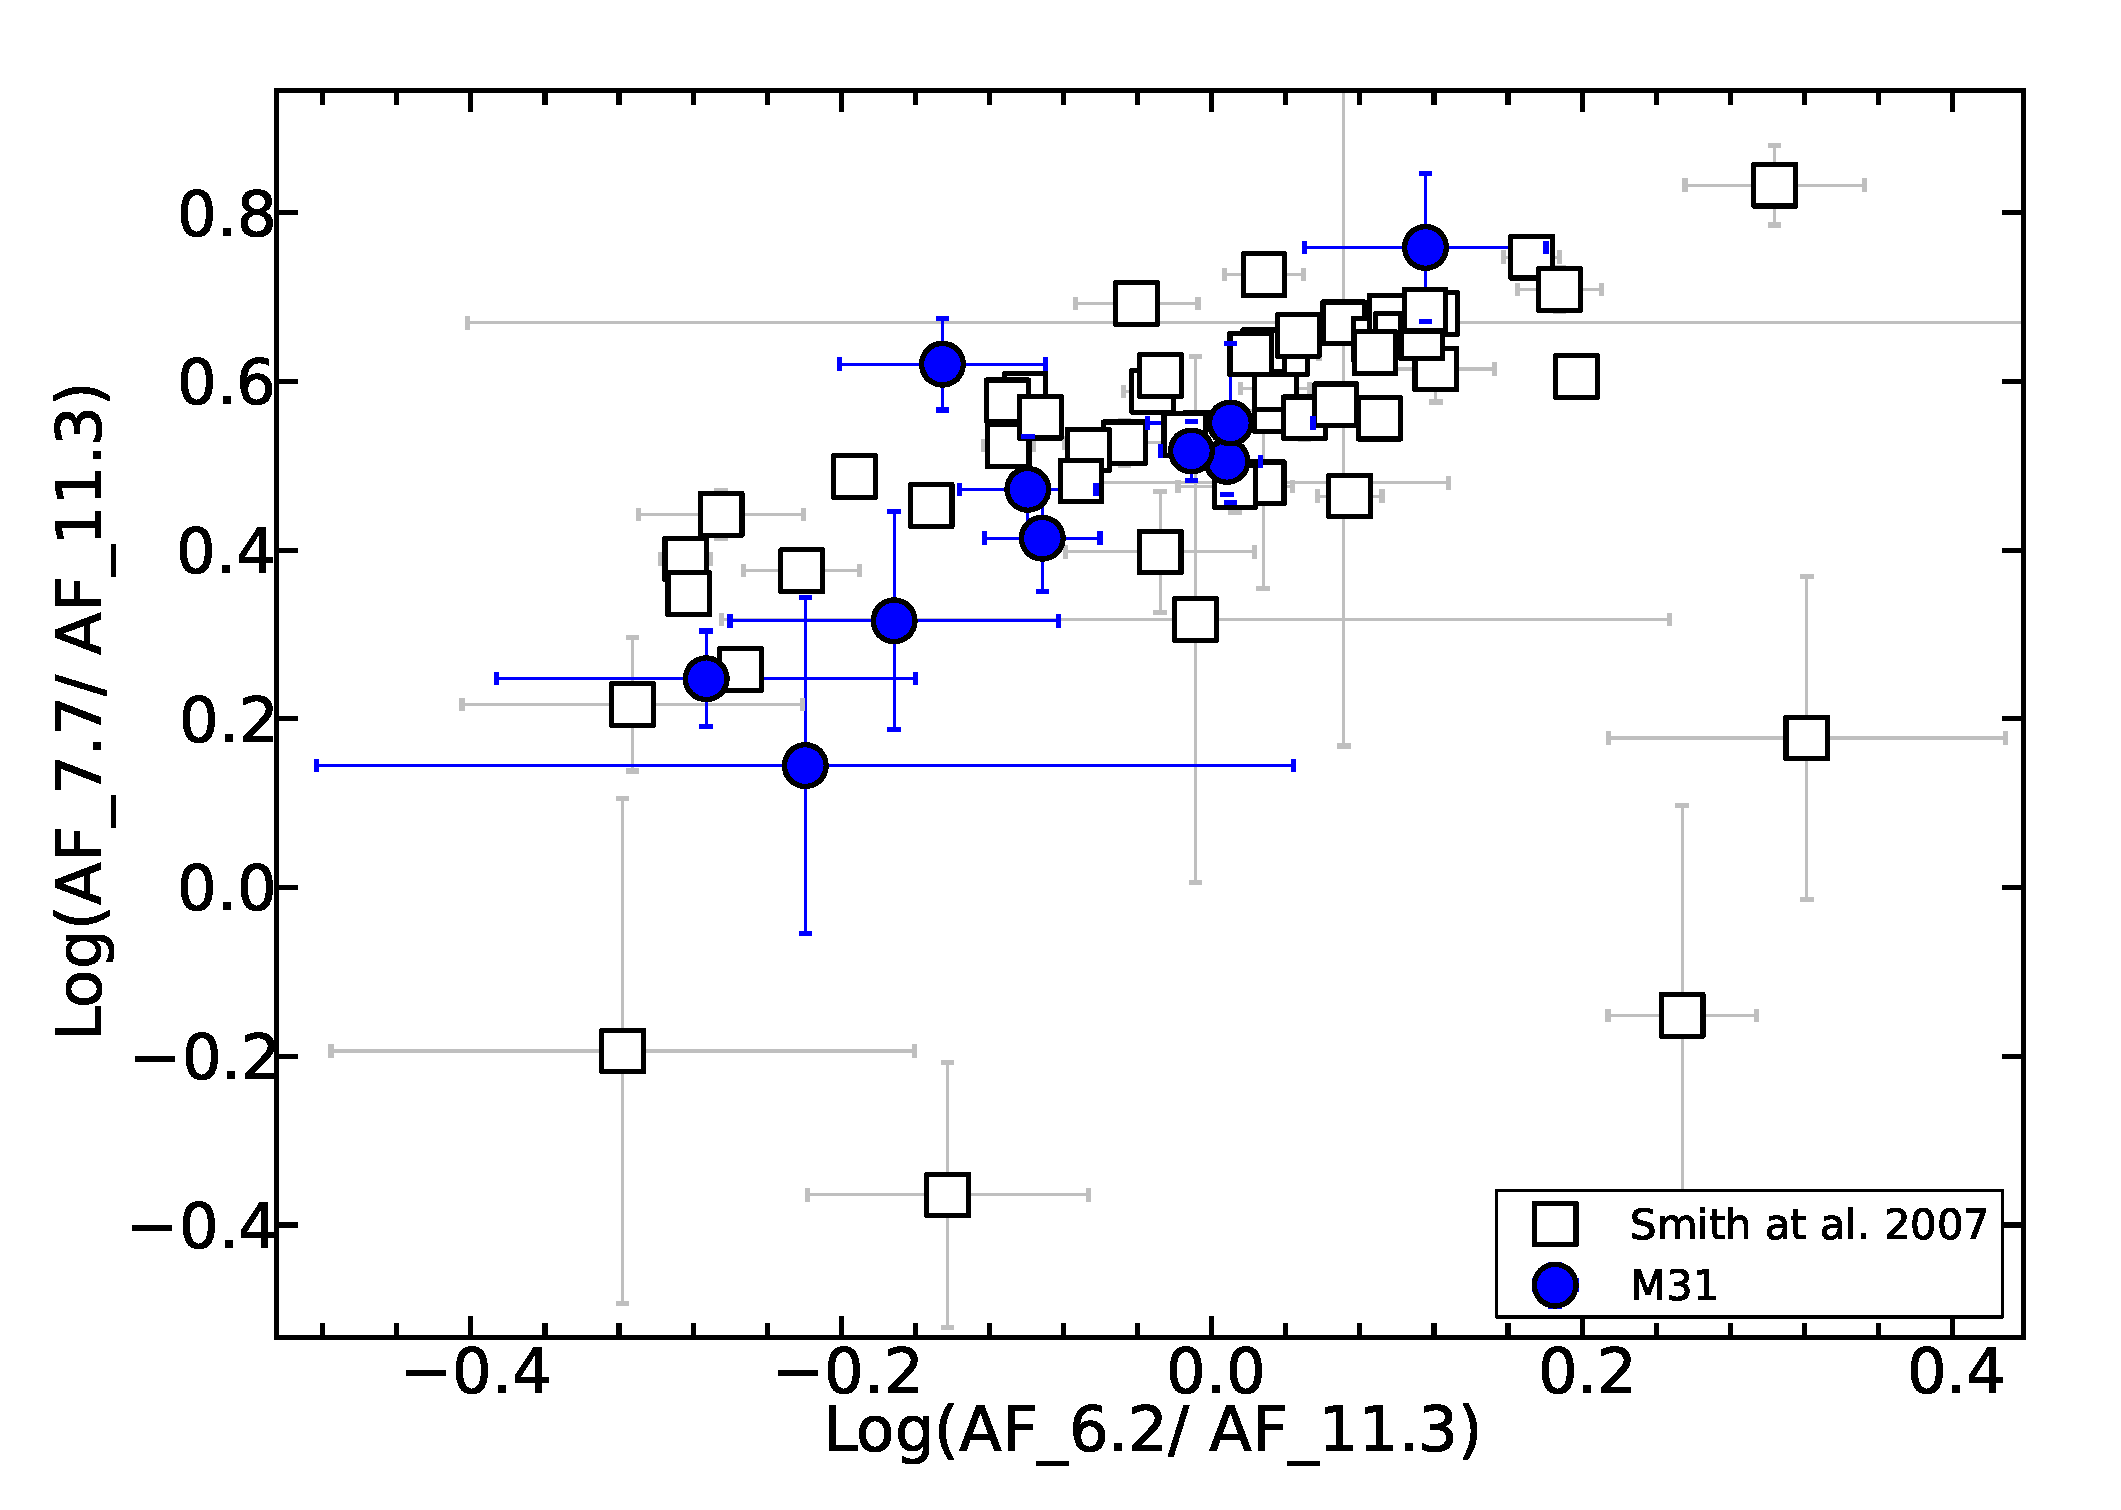
\includegraphics[scale = 0.25]{./SINGSnMy.eps}
\caption{ Flux ratios of 7.7/11.3 vs 6.2/11.3 PAH features from the regions of our sample.}
%\end{center}
\label{PAHlines}
\end{figure}

\subsection{Aromatic EQWs vs Radiation Hardness }
\begin{figure}

\centering
%\begin{center}
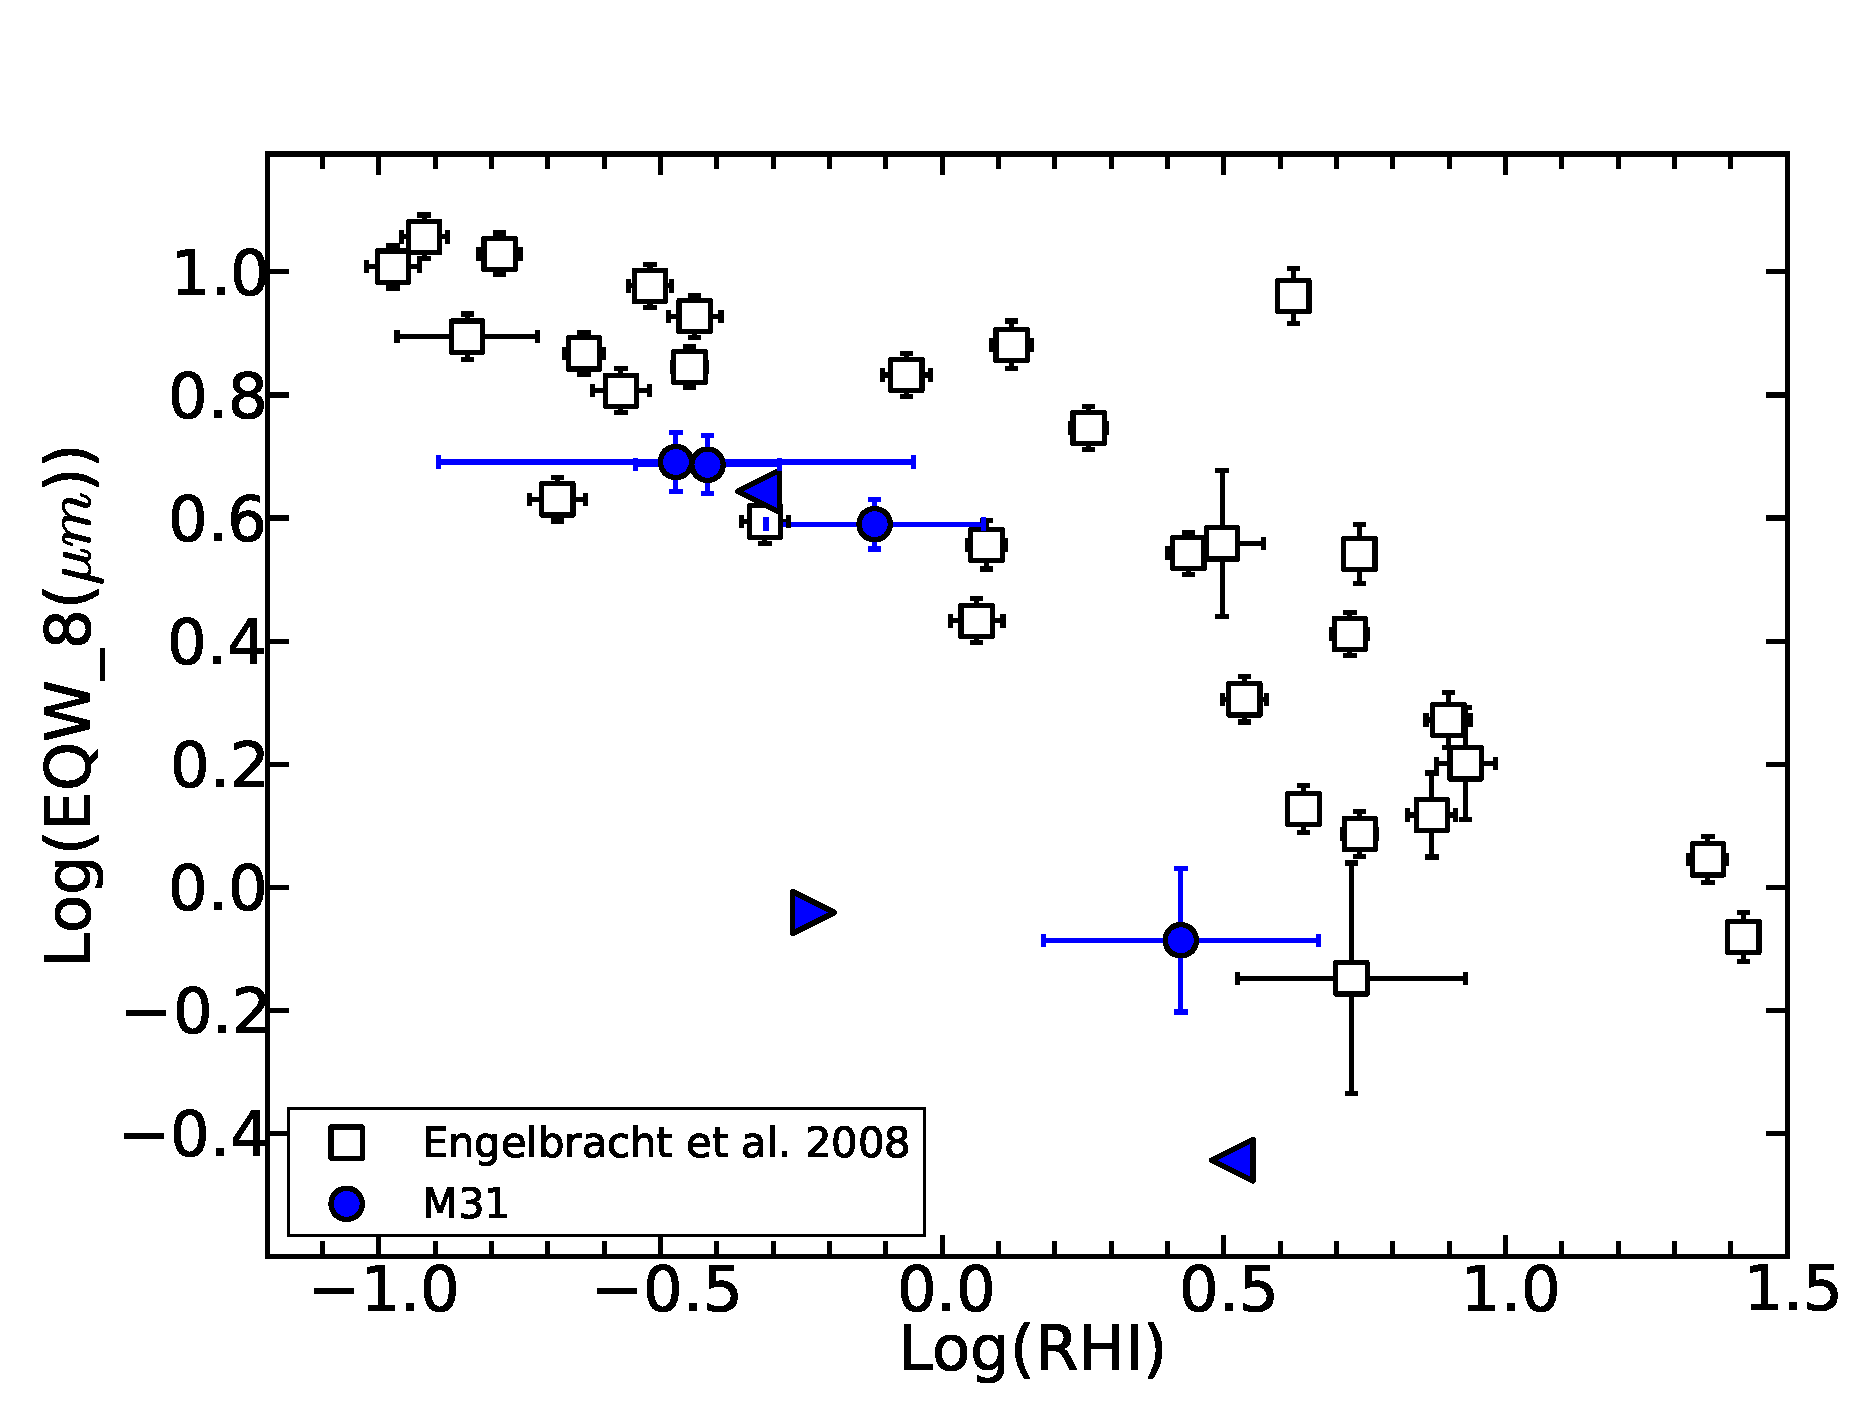
\includegraphics[scale=0.25]{./englvsmy.eps}
\caption{ Equivalent widths of the 8 $\mu$m aromatic feature are plotted vs RHI for our sample (blue). Open squares represent the starburst sample from \citet{Engelbracht_2008}. Here the 8$\mu$m feature is a combination of the 7.7, 8.3 and 8.6 $\mu$m PAHFIT components. Triangles represents the upper and lower limits.}\label{II}
\label{englII}

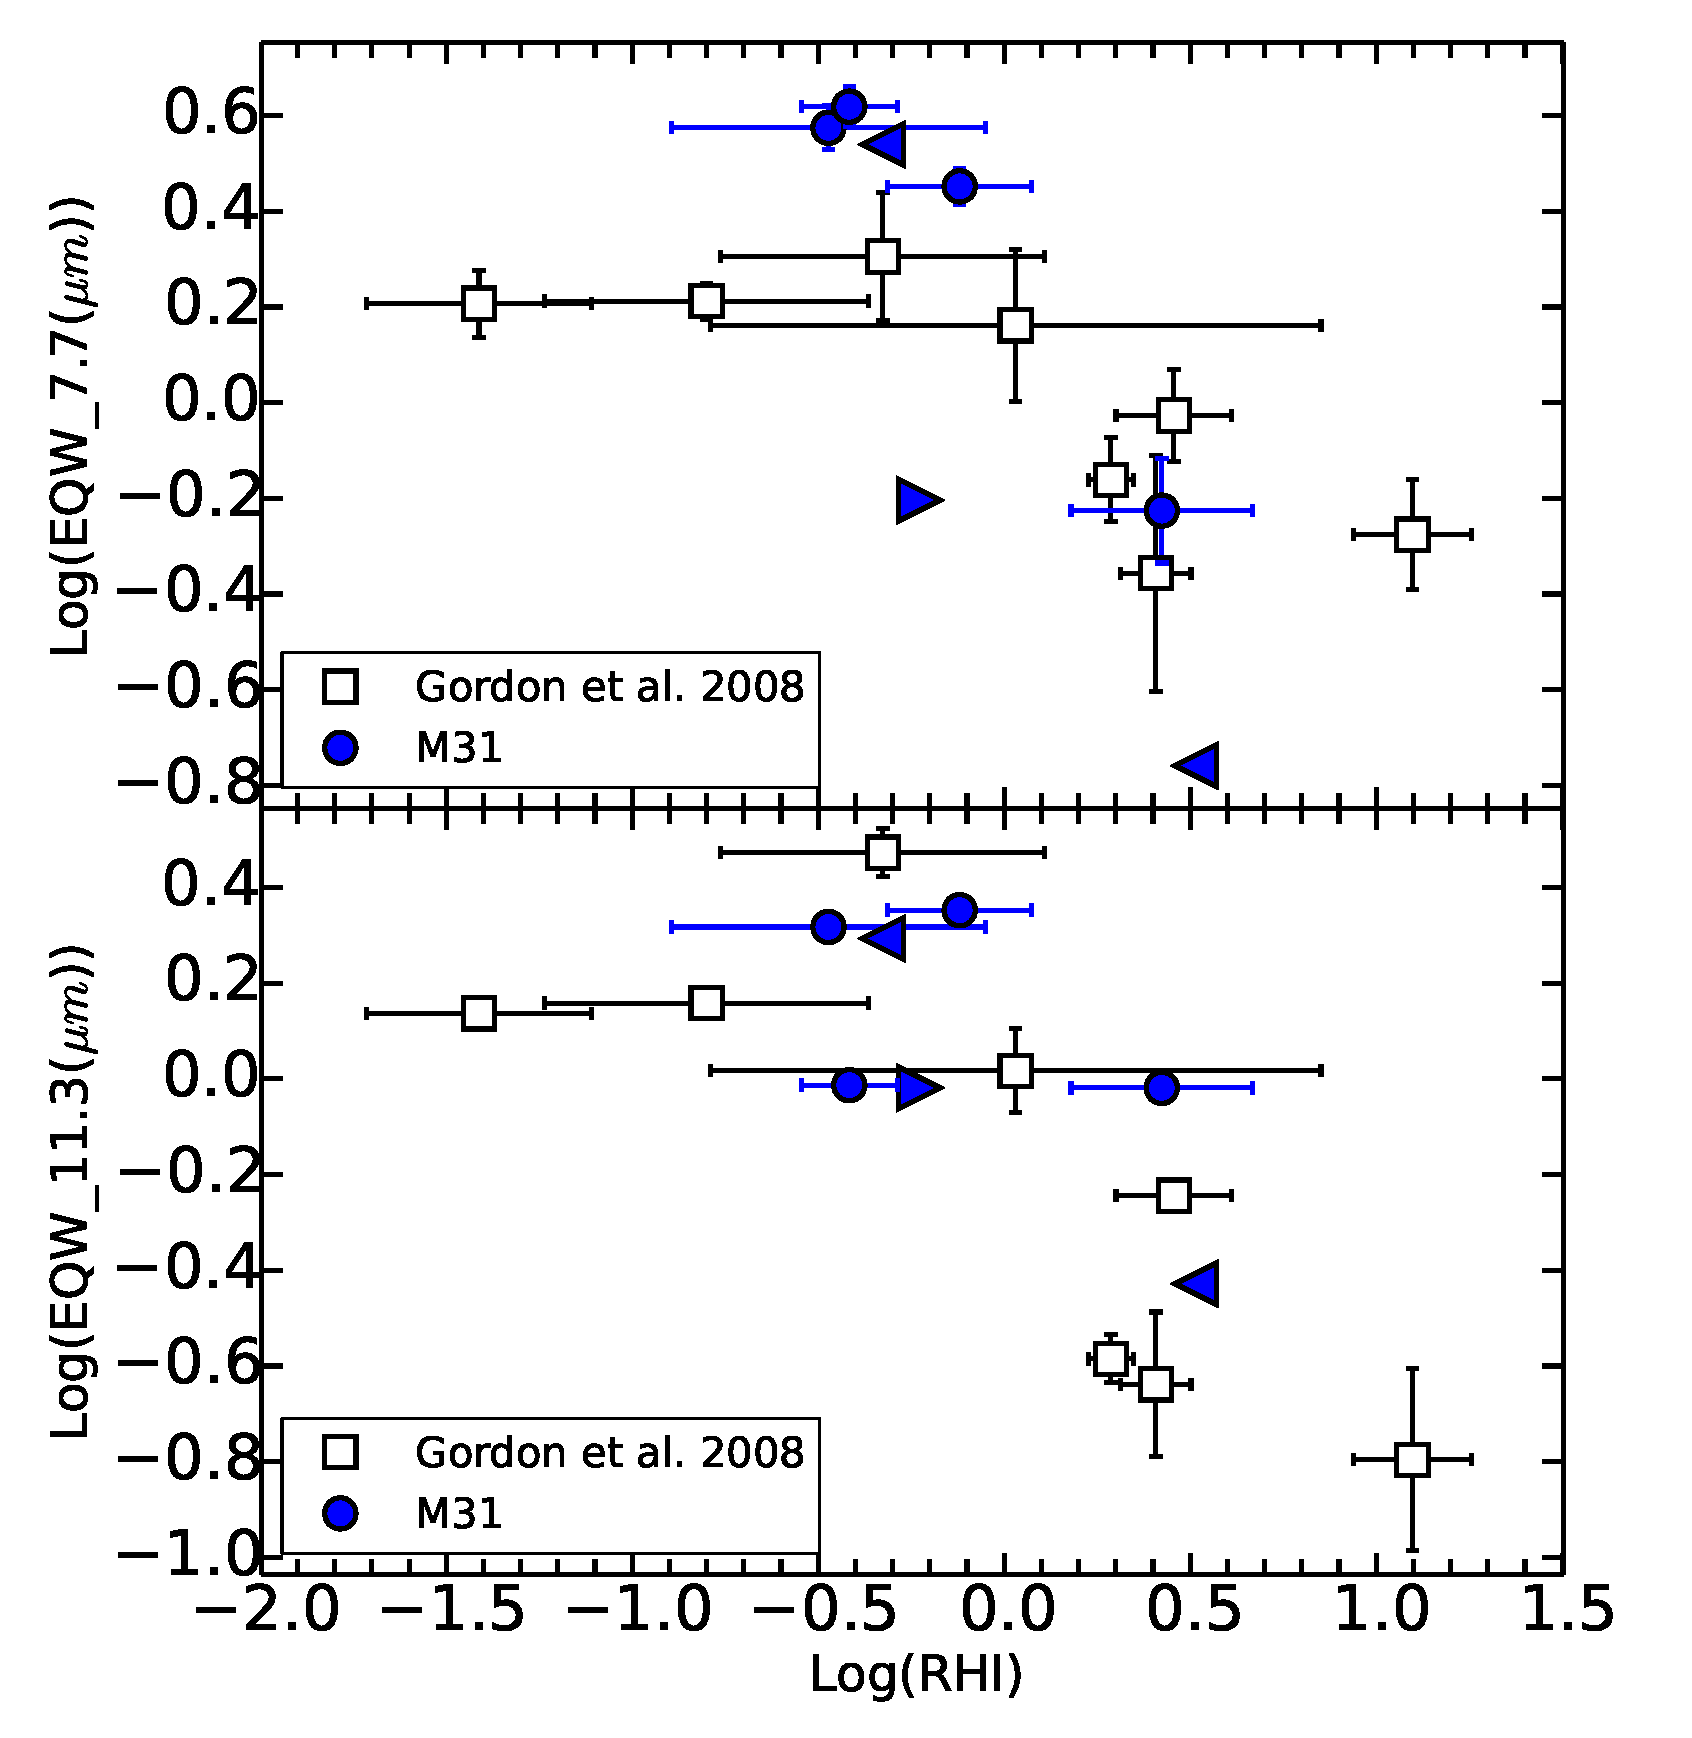
\includegraphics[scale=0.30]{./Gordvsmy.eps}
\caption{ The equivalent widths of the normalized 7.7 $\mu$m aromatic feature (top panel) and 11.3 $\mu$m aromatic feature (bottom panel) are plotted vs RHI for our sample (blue). Open squares represent the data from M101 by \citet{Gordon:2008lr}. The normalization was done by dividing each EQW by the weighted average over all regions in the respective samples. Triangles are the upper and lower limits.}
\label{gordII}
%\end{center}

\end{figure}

As mentioned in the introduction, aromatic equivalent widths tend to show an inverse correlation with radiation hardness. We used the radiation hardness index (RHI) values calculated using the method described in section 3.4 to study how the EQW values from our sample agree with this.

The equivalent widths of the PAH features are compared with RHI in Figures \ref{II} and \ref{gordII}.
For reference, we have added this to the starburst sample of \citet{Engelbracht_2008} and the H~{\sc ii} regions in M101 of \citet{Gordon:2008lr}. The equivalent widths seems to be decreasing with increasing radiation hardness, consistent with previous results. This also helps to confirm that the aromatic emission in M31 is not unusual. 

Atomic line intensities depend on the distance from H~{\sc ii} region to the extraction region used to obtain a spectrum.(\citealt{Dave2014}, in prep.). For an example, [Ne~{\sc ii}]  line intensity can be higher from an extraction close to the H~{\sc ii} region than from an extraction further away. Our maps are at different distances from H~{\sc ii} regions. Therefore the calculated RHI values must have been affected by this.


\subsection{Aromatic EQWs vs Metallicity }


Many studies based on ISO and {\em Spitzer} observations have reported that PAH intensity decreases with decreasing metallicity \citep{Calzetti:2010fk}. In addition, these studies also report a sudden drop of EQWs of PAHs around 12+log(O/H) $\approx$ 8.1 where 12+log(O/H) is a measure of metallicity. This has been observed amongst different galaxies \citep{Engelbracht_2008} as well as within a single galaxy \citep{Gordon:2008lr}. 

Here we investigate the relation between the PAH features and the metallicity for the M31 regions in this paper. \citet{Sanders_2011} provided metallicities for more than 250 H~{\sc ii} regions and this catalogue was used to find the metallicity values for the regions of interest in this paper. Except for two regions (Region 5, Region 8), we found the metallicity values for all the regions under the strong line diagnostic method of N06 N2 described in \citet{Sanders_2011}. This method uses  [N~{\sc ii}]/H$\alpha$ and  [O~{\sc iii}]/[N~{\sc ii}] oxygen abundance callibrations of \citealt{Nagao2006}. \citet{Sanders_2011} also provided a radial metallicity profile of M31 based on the N06 N2 method which we used to find metallicity values for Region 5 and Region 8. Our regions do not cover metallicity values less than 8.40 (see Table 1).


\begin{figure}

\centering
%\begin{center}
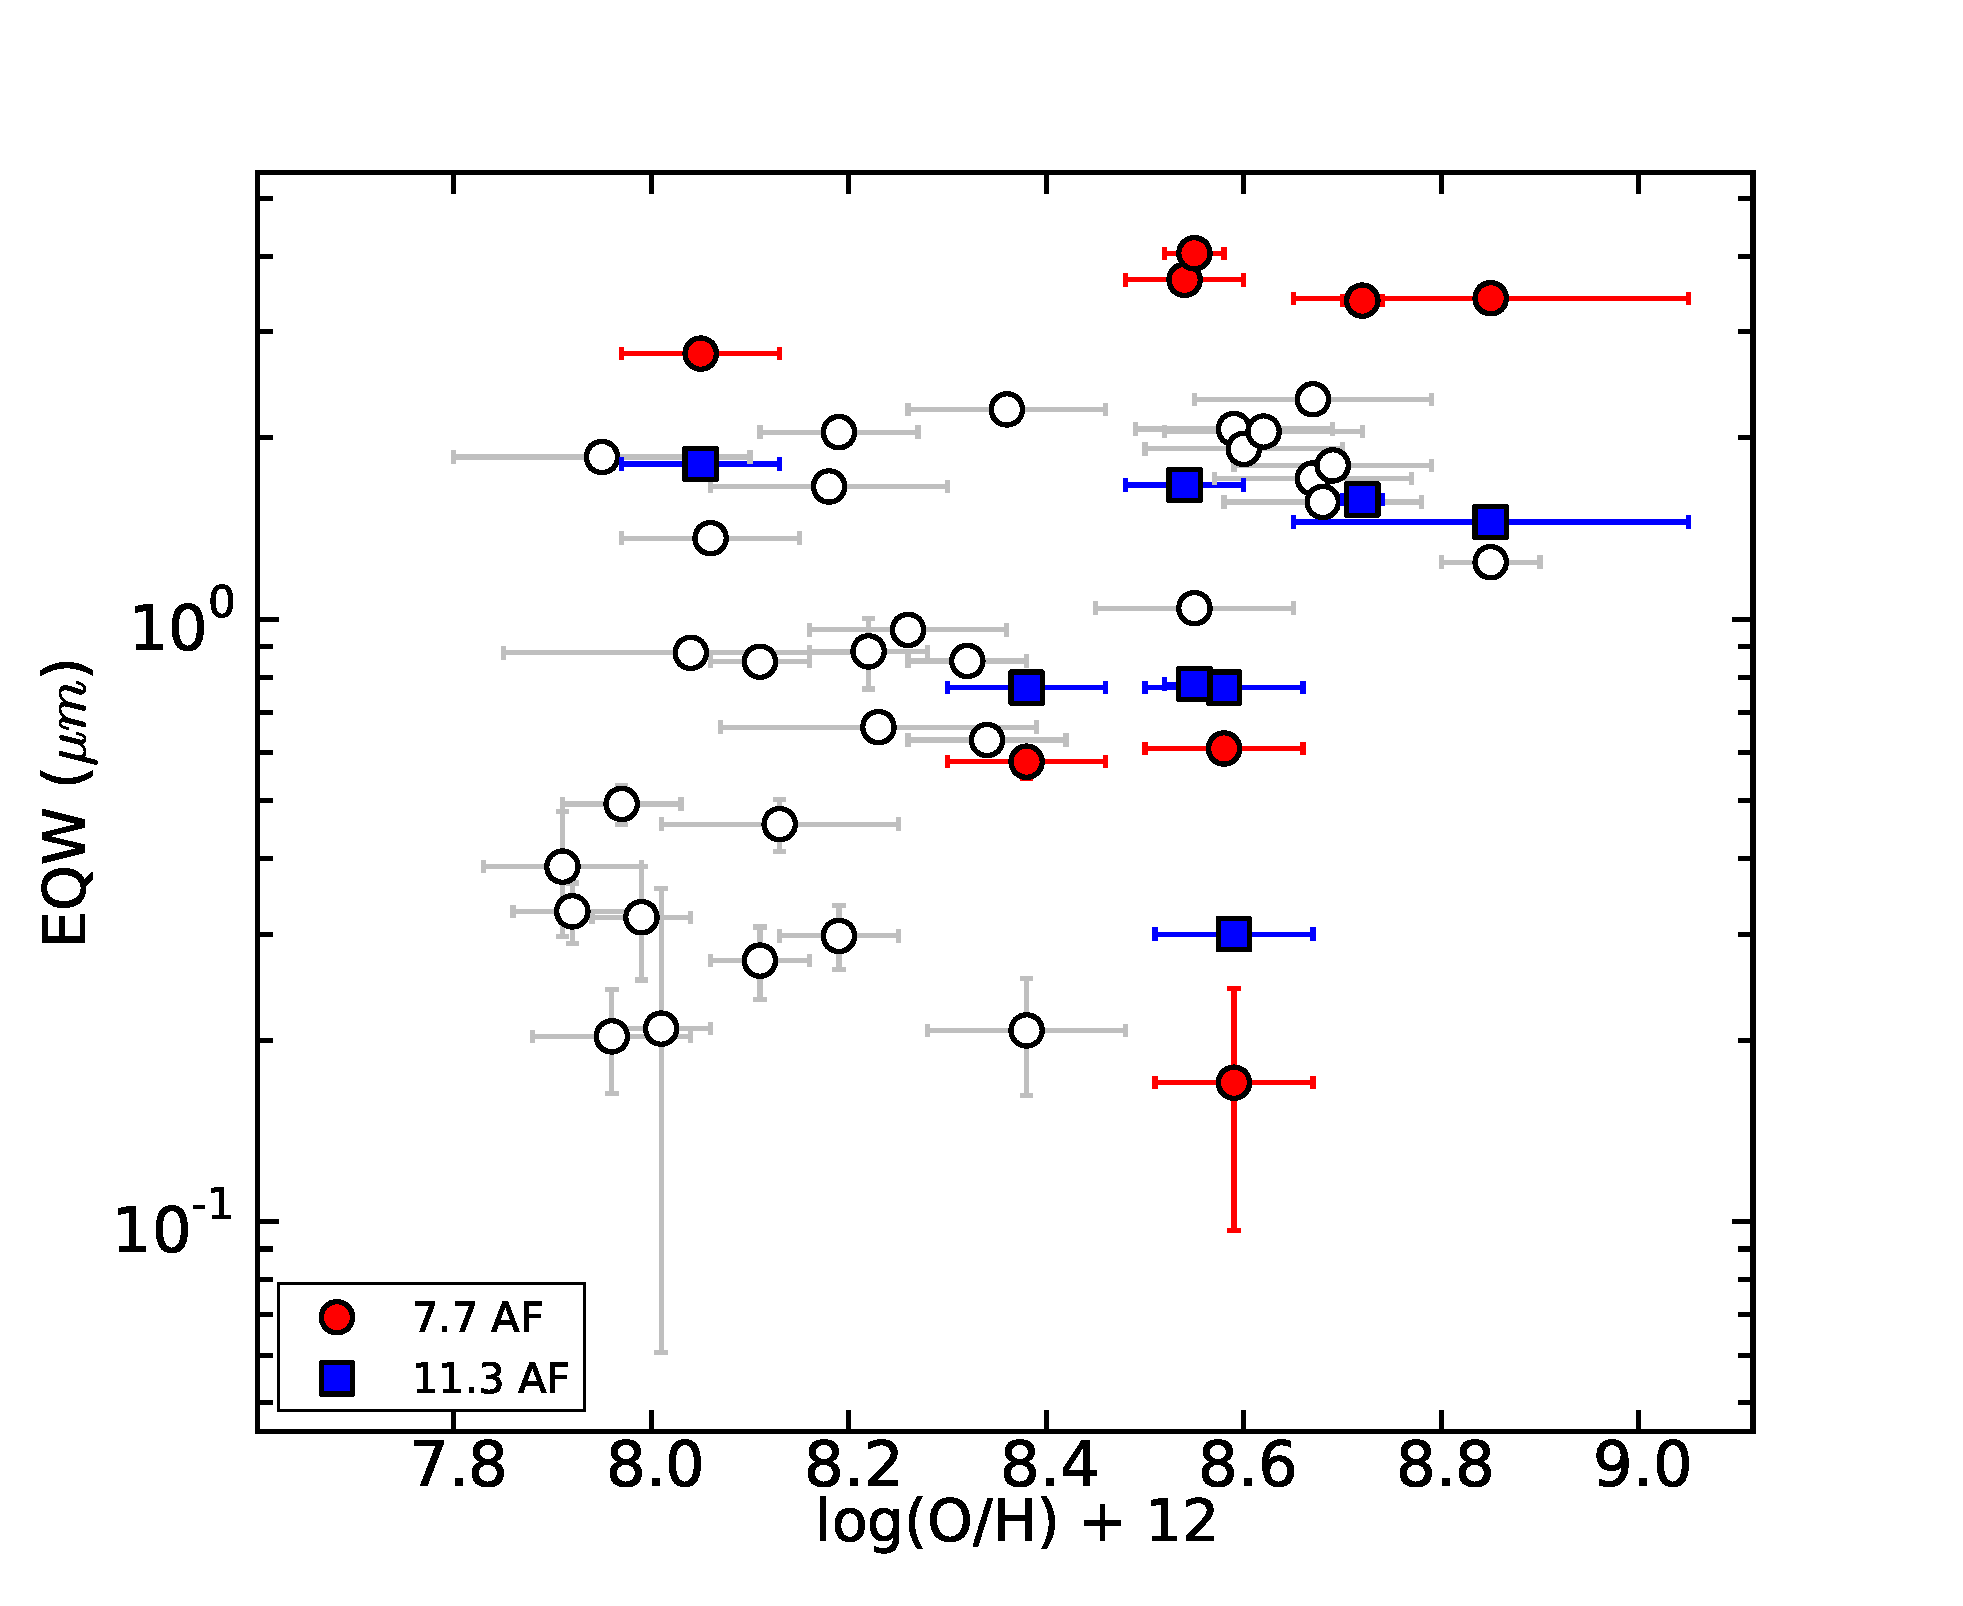
\includegraphics[scale=0.27]{./oxyvseqw.eps}
\caption{ PAH EQWs vs metallicity. EQWs of the 7.7 $\mu$m feature of the starburst sample from \citet{Engelbracht_2008} are plotted in open circles.}
%\end{center}
\label{metalicityVseqw}
\end{figure}

	The normalized EQWs of the PAH features are plotted versus the metallicity in our sample and the starburst galaxies of \citet{Engelbracht_2008} in Figure \ref{metalicityVseqw}. The metallicities in Engelbracht's work have been obtained by the direct electron temperature method \citep{Skillman1998} whereas we used N06 N2 method. There is an offset between the metallicities generated by these two methods since the N06 N2 method gives slightly higher values for the metallicity than the direct method. This offset has been calculated by \citet{Mitchel2014} to be 0.35$\pm$0.10. In Figure \ref{metalicityVseqw} we have corrected for this offset by subtracting our metallicity values by 0.35. 
	
	Equivalent widths of the 7.7 and 11.3 micron features are not inconsistent with Engelbracht's. But we do not have enough data from low metallicity regions in M31 to observe the expected decrease of EQWs of PAH with the decreasing metallicity.  There do seem to be some outliers which can plausibly be due to the uncertainties  and the offset between different methods of calculating the metallicity.  



\begin{figure}

\centering
%\begin{center}
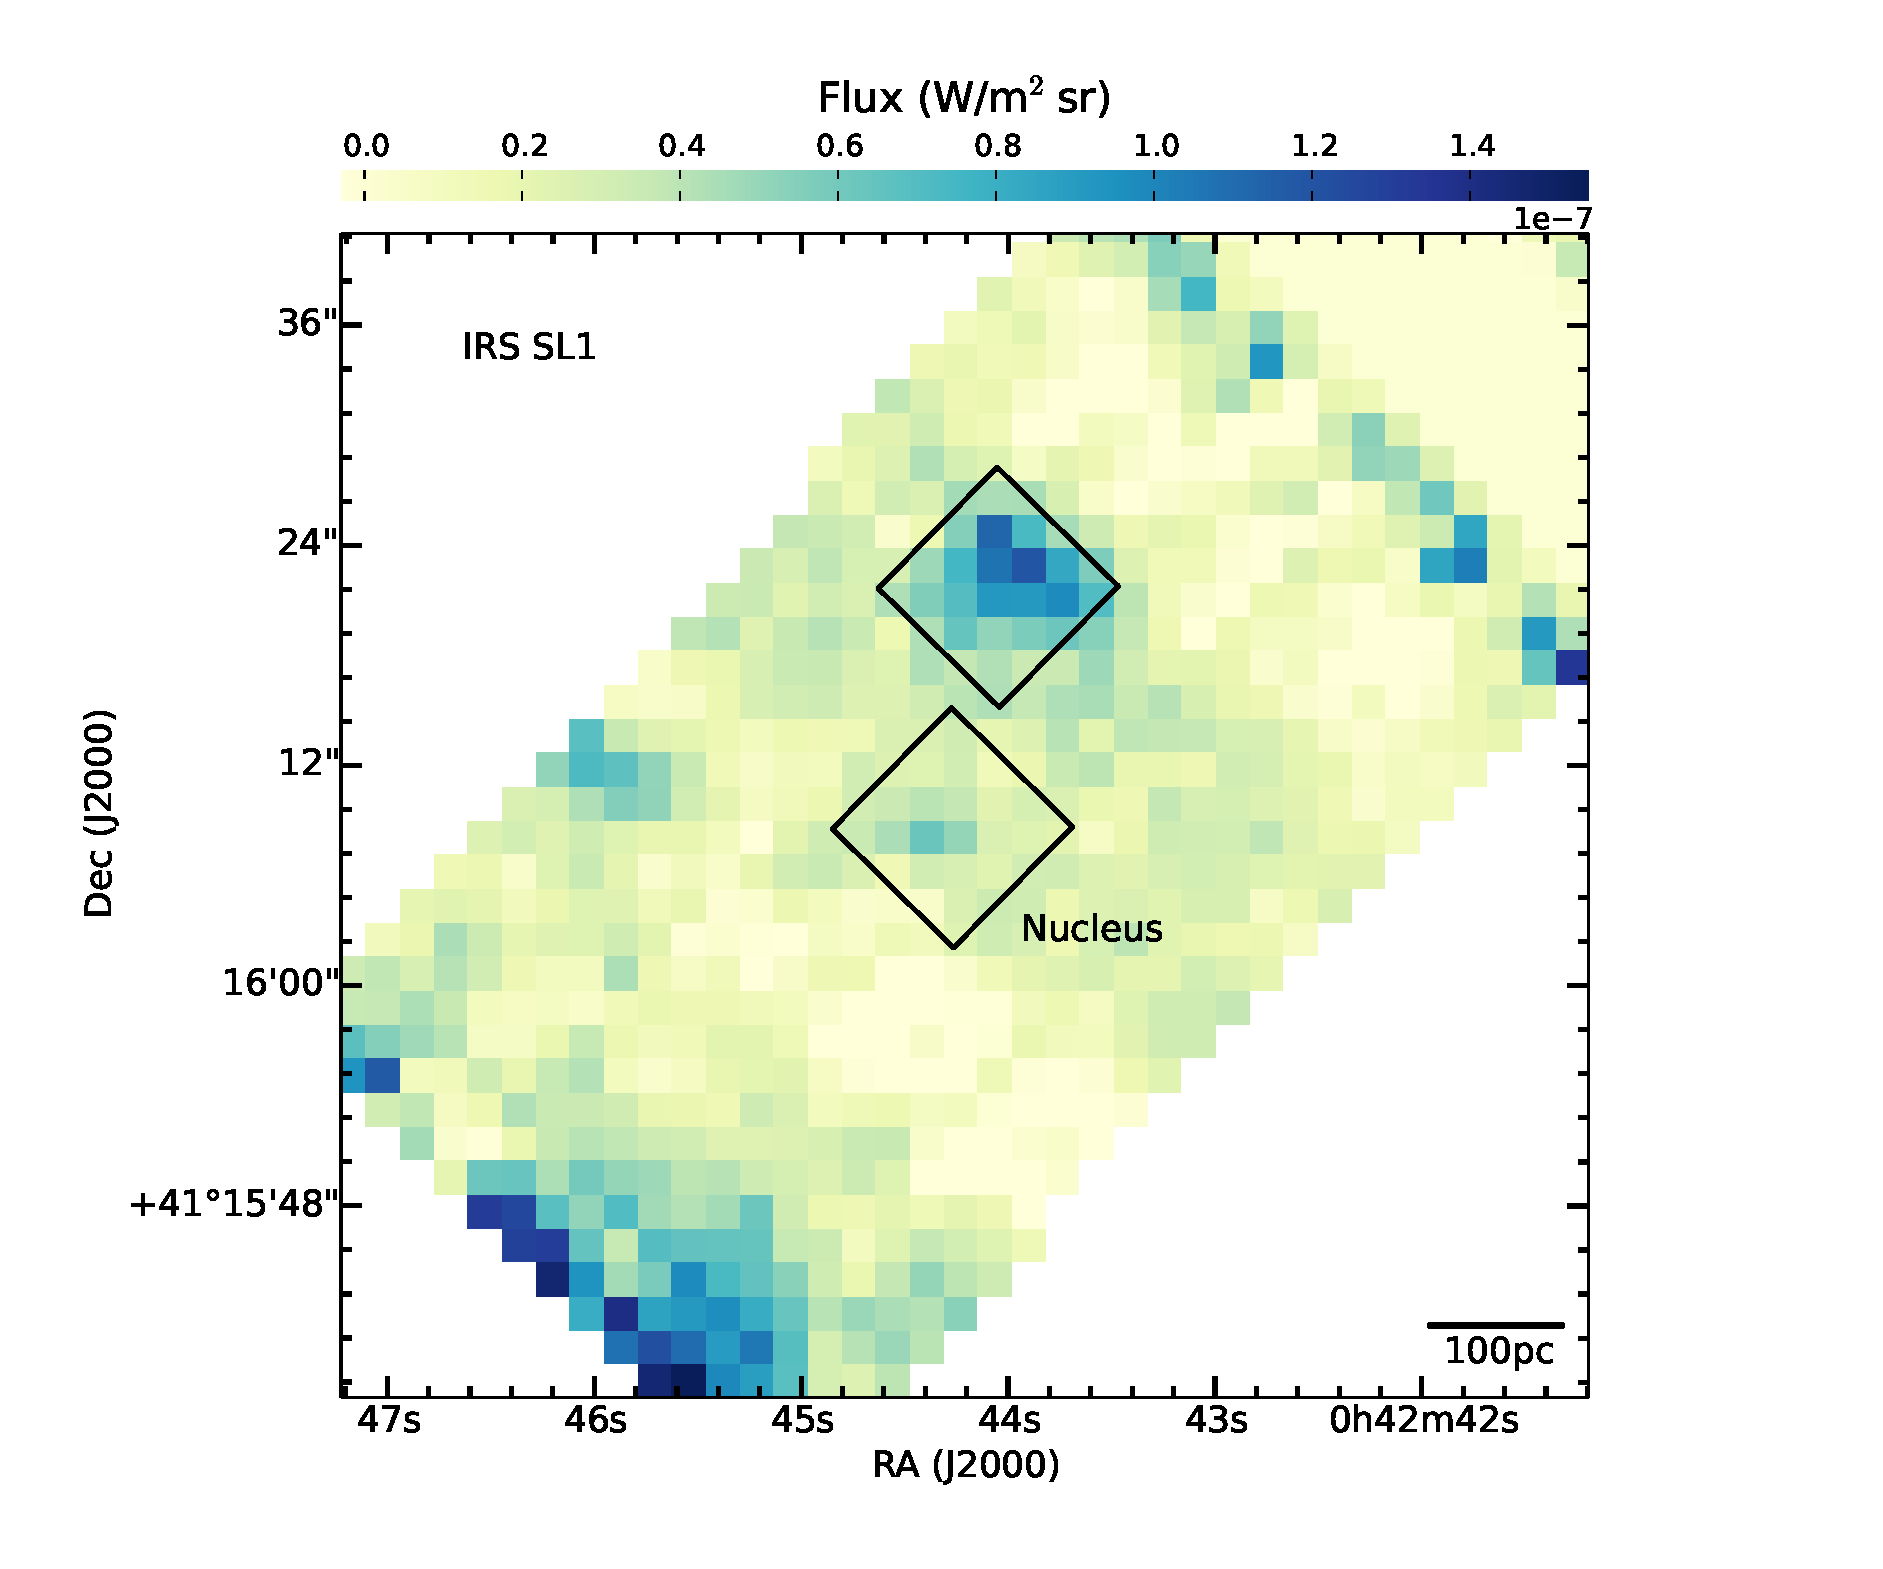
\includegraphics[width = 8 cm]{./nuc11_3.eps}
\caption{ Intensity variation of 11.3 $\mu$m emission around the nucleus of M31. Two black boxes are the apertures (centre and the north region) that used to extract spectra in Figure \ref{smithspec}. The centre of the nucleus is at R.A. 0h42m44.35s, Dec. +41d16m08.5s \citep{NucleusREF}.}
%\end{center}
\label{nuc11}
\end{figure}

\subsection{Dust properties of the nucleus }

\begin{figure*}

\centering
%\begin{center}
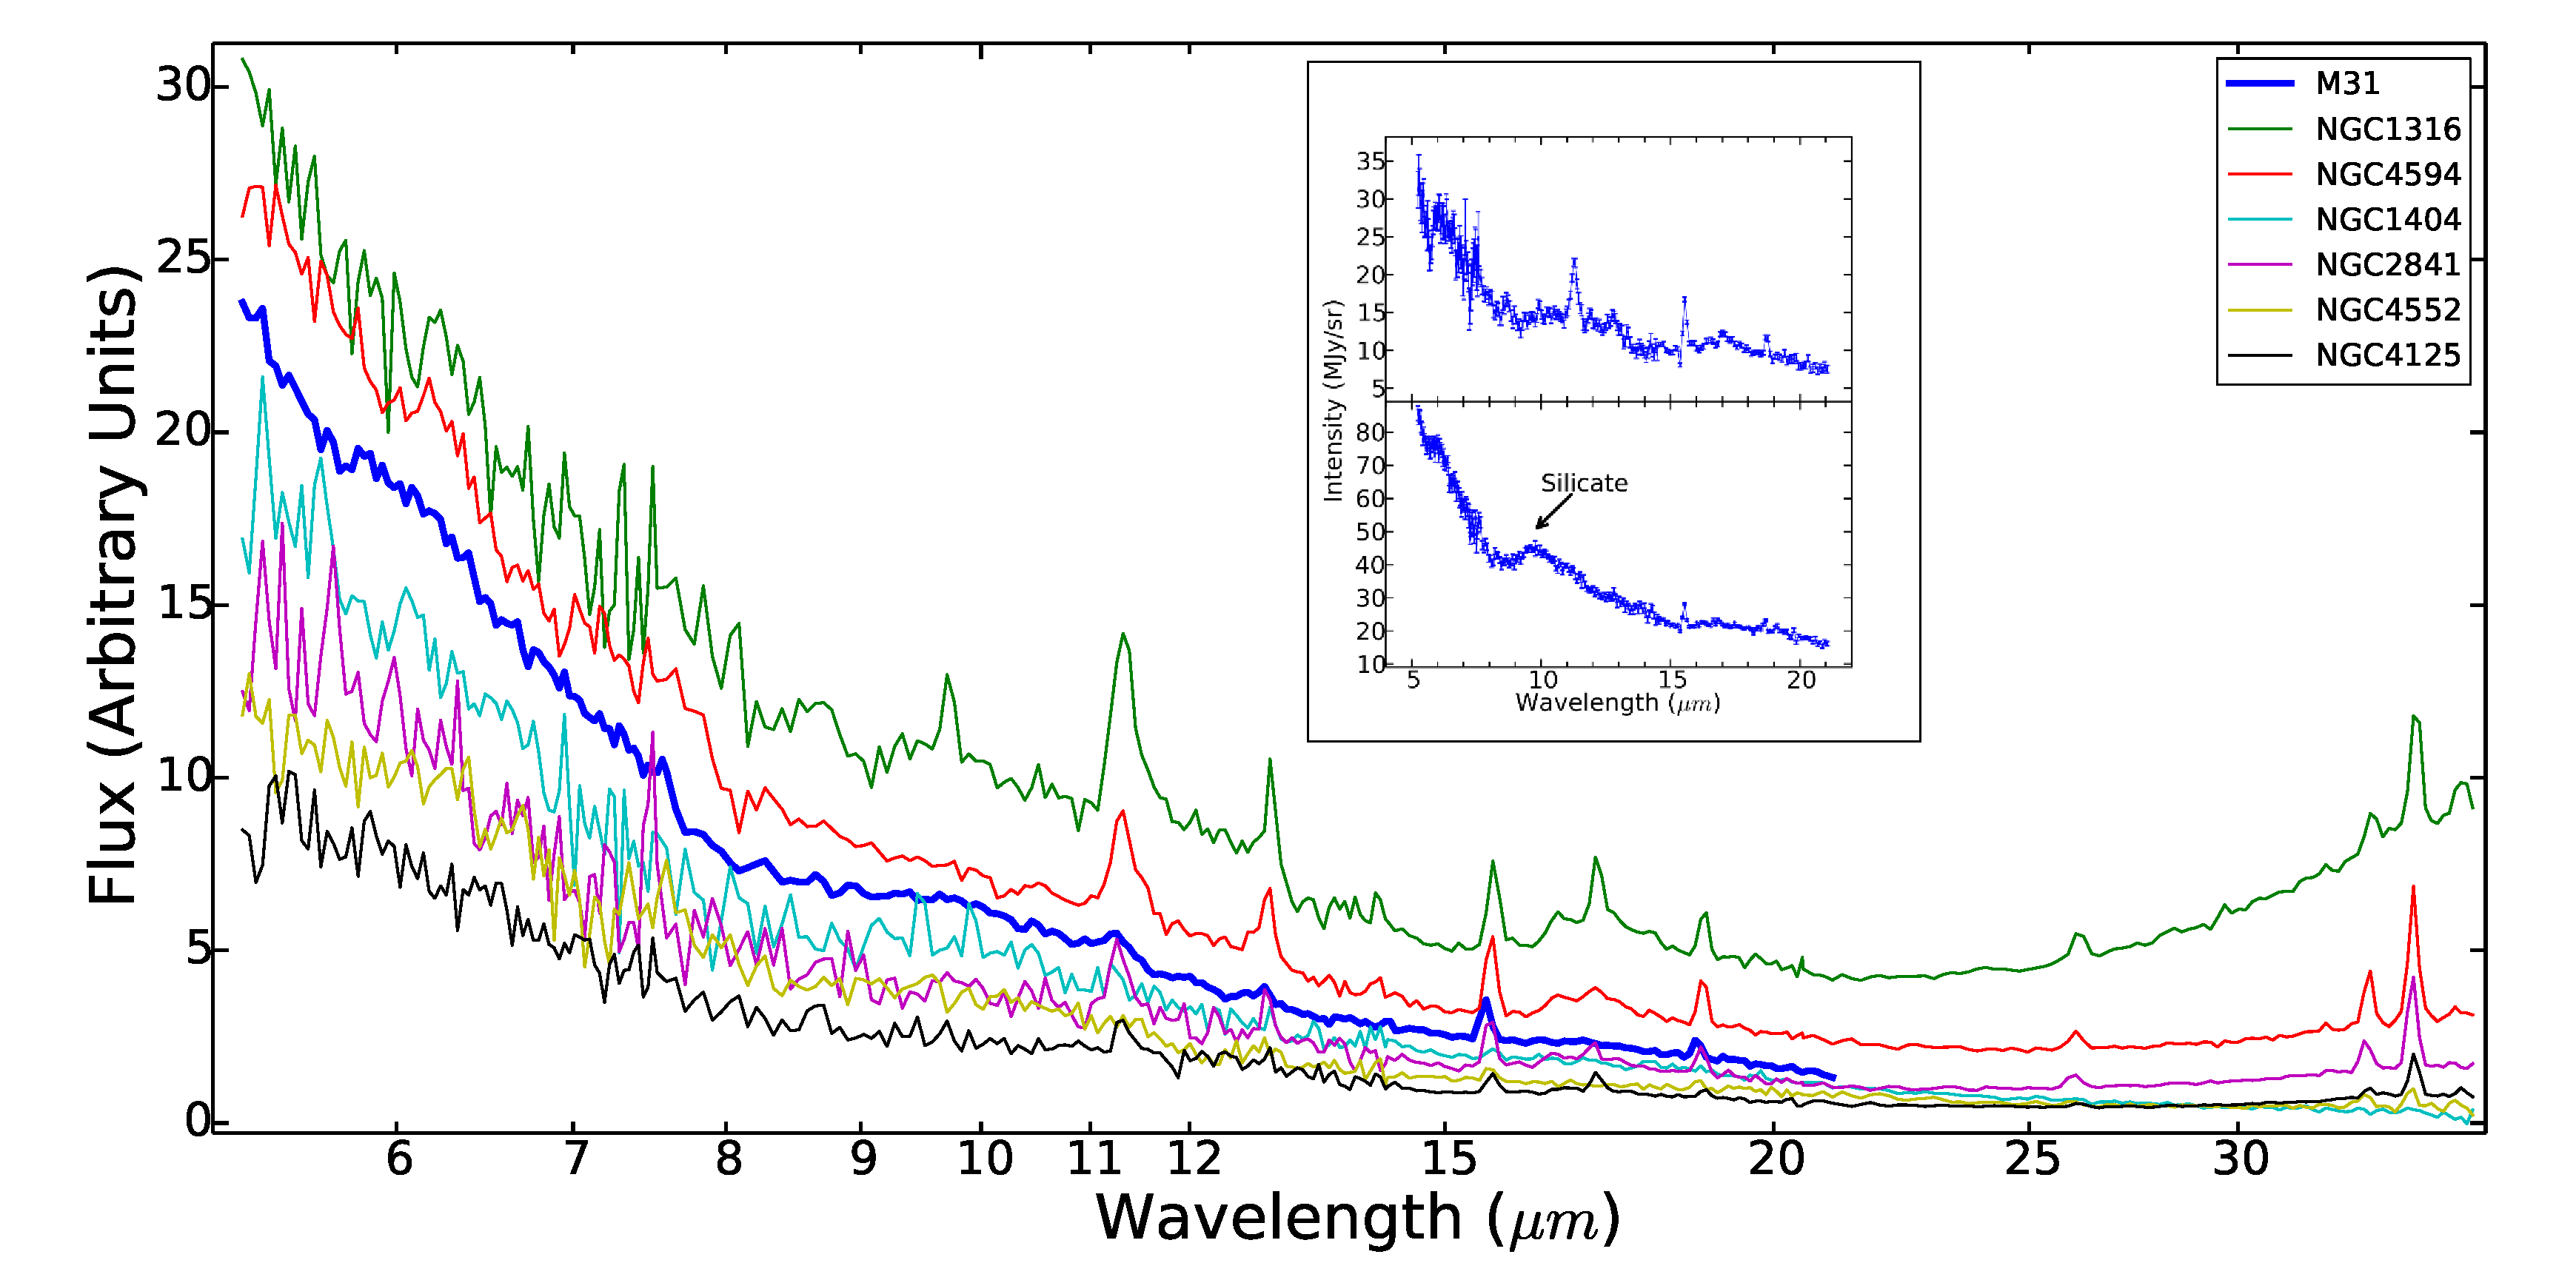
\includegraphics[height = 8 cm]{./SINGSspec.eps}
\caption{ Spectrum from the nucleus of M31 (blue) over plotted with spectra extracted close to the nucleus of 6 nearby galaxies which have AGN activity \citep{Smith:2007lr}. NGC 4552, NGC 1404 and NGC 4125 are elliptical galaxies and NGC 4594 and NGC 2841 are spiral galaxies. NGC 1316 is a lenticular galaxy. The inset shows the spectra extracted from the centre region of the nucleus (bottom) and from the north region (top) shown in Figure \ref{nuc11}.}
%\end{center}
\label{smithspec}
\end{figure*}

	
The centre of M31 has a complicated physical structure. It hosts a very inactive supermassive black hole with  mass of 0.7-1.4 $\times$ 10$^8$ M$\sun$ \citep{Bacon2001} and it also has a lopsided nuclear disk \citep{Lauer1993} with two stellar components and an A-star cluster. The spectra of the nucleus from both {\em Spitzer} and ISOCAM show similar characteristics in the mid infrared wavelengths. Emission from the nucleus is missing the most common 6 to 8 $\mu$m PAH features while showing considerable emission around 11.3 $\mu$m. 

A suppression of 6 to 8 $\mu$m features has also been observed in other nearby star-forming galaxies with a low-luminosity AGN \citep{Smith:2007lr}. One explanation for this behaviour is that the AGN environment can selectively destroy the ionized or small PAH molecules which contribute to the 6 to 8 $\mu$m features (whereas larger, neutral PAHs contribute to the 11.3 $\mu$m feature). Another argument is that the AGN is unrelated or partially responsible for the PAH spectra alterations. \citet{Smith:2007lr} argue that this variation could be used to detect weak AGNs in dusty galaxies where optical diagnostics are not available. In Figure \ref{smithspec} we compare the spectrum of the nucleus of M31 with spectra extracted close to the nucleus of 6 other nearby galaxies and they all look very similar. All six galaxies are known to have low luminosity AGNs (LLAGNs) in the centre. Since M31 is showing a similar spectrum from the nucleus we can infer that the M31 also has a weak AGN at the centre.

Figure \ref{nuc11} shows the integrated intensity map of 11.3 $\mu$m emission around the nucleus. It can be observed that the majority of the 11.3 $\mu$m emission is coming from two regions (North and South East) around the centre of the nucleus and lacks at the centre. To study this further, we extracted two spectra, one from the centre and one from the North region using a 5 $\times$ 5 pixels square aperture as shown in Figure \ref{nuc11}. The spectrum extracted from the North region shows a strong 11.3 $\mu$m peak as expected and no considerable emission from 6 to 8 $\mu$m features (Figure \ref{smithspec}, inset). On the other hand the centre shows no PAH emission (Figure \ref{smithspec}) but silicate emission around 9.7 $\mu$m which is not present in the other spectrum. To investigate whether there are any other regions that show silicate emission close to the nucleus, a continuum subtracted image was produced which shows the 9 to 11 $\mu$m integrated silicate emission intensity (see Figure \ref{silicate}). This silicate emission map shows that only the exact centre of the nucleus contributes to the silicate emission. 

\citet{Spoon2007} report that galaxies which have AGN activity show silicate emission around 9.7 $\mu$m.
In the unified model of AGNs, an edge on view through cool dust (type 2 AGNs) in the torus causes silicate absorption whereas a face on view (type 1 AGNs) shows silicate emission \citep{AGNtypes1995}. The latter could be the reason for silicate emission of M31 if it holds a Seyfert like AGN. But the mid-IR spectra do not contain forbidden atomic lines such as [Ne~{\sc v}] and [S~{\sc iv}] which are indicative of such an active nuclei \citep{AGNref}.

 Alternatively, the silicate emission is not directly associated with the torus but rather originate in the optically thin hot dust around the torus \citep{Mason2012}. The first detection of such silicate emission is reported in \citet{Sturm2005} from the low-ionization nuclear emission-line region (LINER) galaxy NGC 3998. LINERS are powered by accretion onto massive black holes and due to the low accretion rates these are classified under the low-luminosity AGNs \citep{Kewley2006}. \citealt{Mason2012} has observed that this 9.7 $\mu$m silicate emission is present in many LLAGNs. They also have explained that these objects can not host a Seyfert-like obscuring torus because of their optically thin dust and low dust-to-gas ratio. By taking all these into account we can suggest that the M31 hosts a low-luminosity AGN. 
 
 Also, the bolometric luminosity of the nucleus was calculated to be (value goes here erg/ s) using the 12 $\mu$m flux using the method described in \citet{luminosity}. This value is closer to that of other LLAGNs.



\begin{figure}

\centering
%\begin{center}
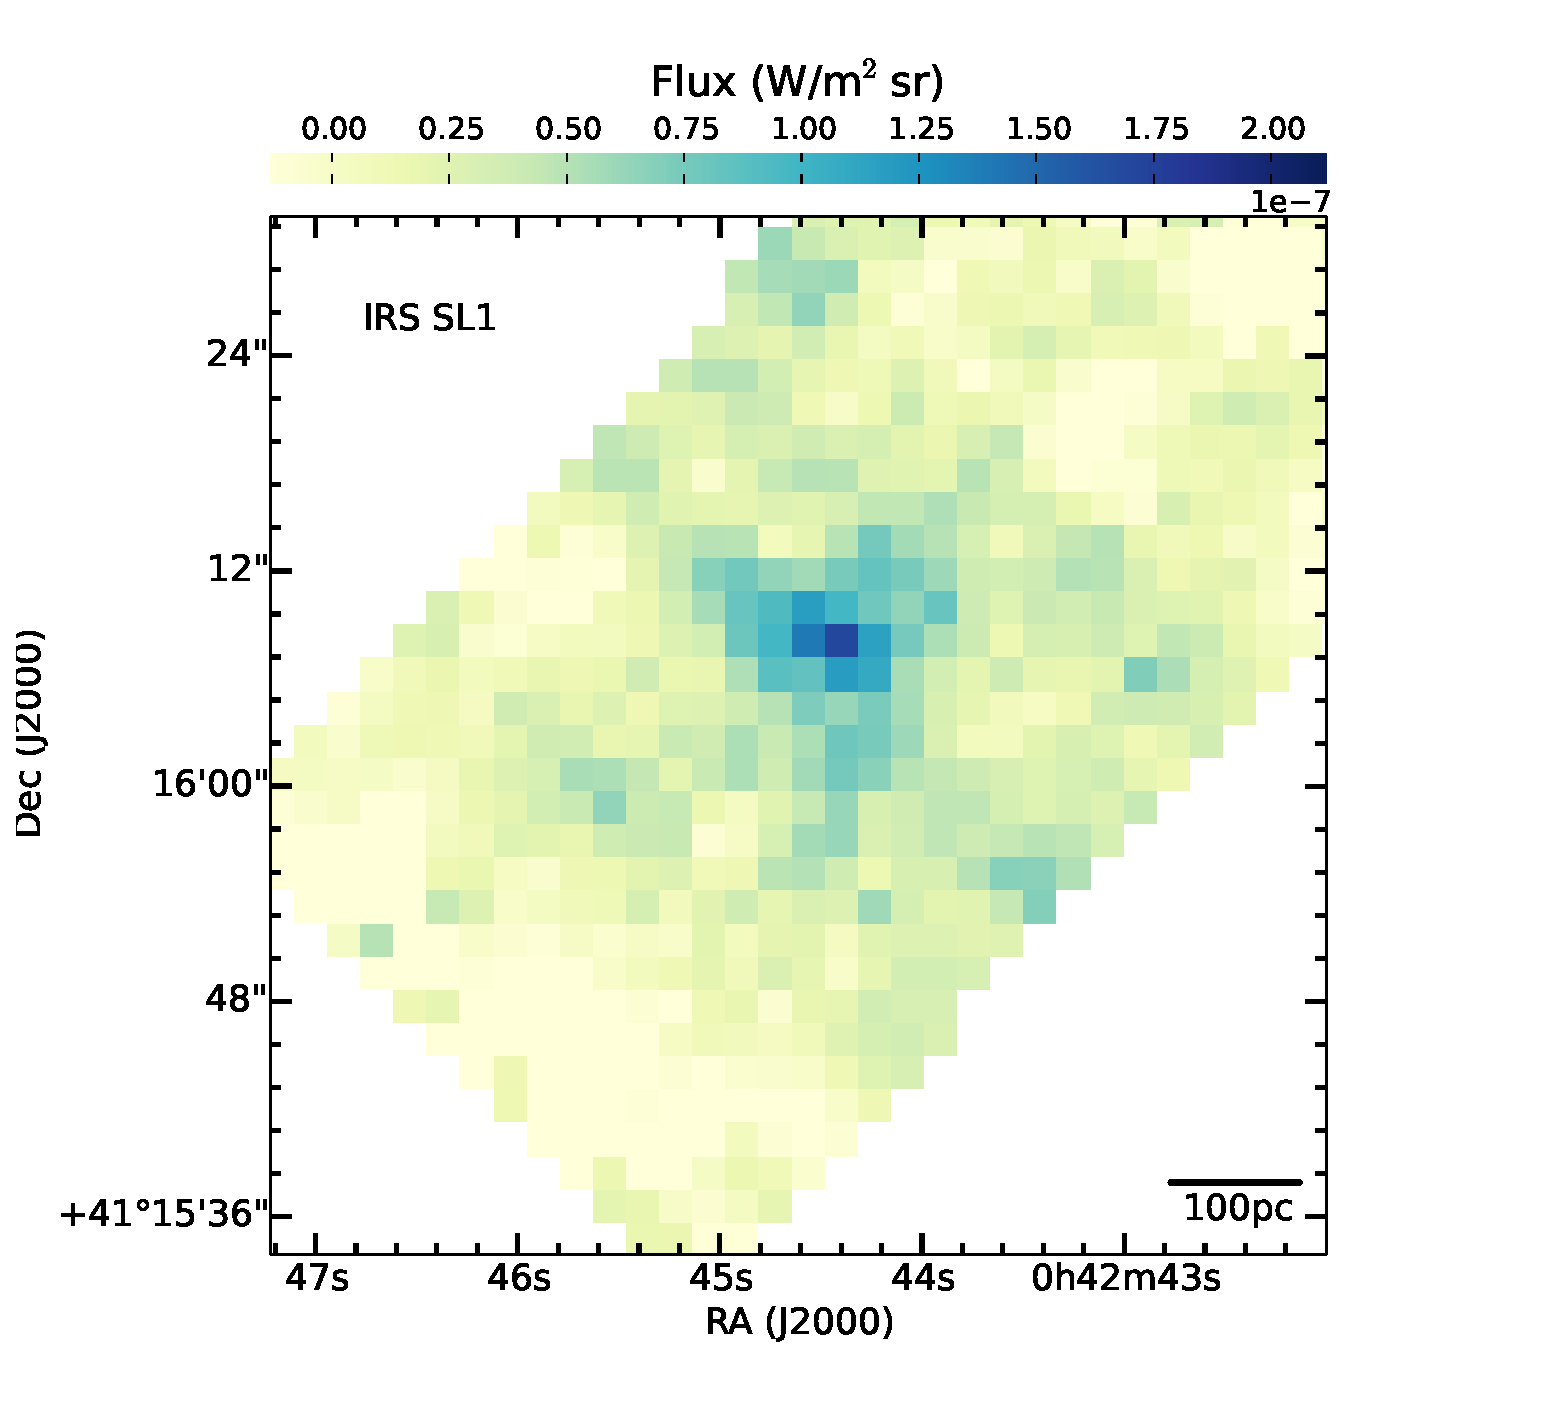
\includegraphics[scale = 0.3]{./NUCsilicate.eps}
\caption{ The integrated strength of the silicate emission around 9 $\mu$m to 11 $\mu$m.}
%\end{center}
\label{silicate}
\end{figure}


\section{Summary and Conclusions}

We have obtained {\em Spitzer}/IRS spectral maps of 12 regions of M31 covering wavelengths from 5 to 21 $\mu$m. The spectra from those regions, except the nucleus, agree with spectra obtained from other nearby  star forming galaxies. But they are inconsistent with previous ISOCAM observations of M31 \citep{1998Cesarsky} reporting a suppression of the 6 to 8 $\mu$m features and an enhancement of 11.3 $\mu$m feature towards 4 regions. Our IRS spectra for three of these ISOCAM regions do not show this unusual behaviour. ISOCAM data corresponding to those three regions in common between our study and that of \citep{1998Cesarsky} were obtained from the ISO archive. These data were reprocessed in 2005 to remove contamination by stray light and zodiacal emission; spectra extracted from these newly processed data could not reproduce previous results. Therefore we conclude that the earlier results based on ISOCAM data were affected by the background subtraction methods applied to overcome the contamination.

PAH equivalent widths showed a decreasing trend with increasing radiation hardness which is consistent with previous results from other nearby galaxies. The PAH EQWs versus metallicity plot did not show a good correlation but the data points were well within the values from the starburst galaxy sample of \citet{Engelbracht_2008}. We did not have enough data from low-metallicity regions of M31 to observe the decreasing trend of EQWs at low metallicity values which is visible in other galaxies.

The mid-IR spectrum from the nucleus was compared with that of six other galaxies which are known to have AGN activity. All have a similar spectral shape and present suppressed 6 to 8 $\mu$m features and a strong 11.3 $\mu$m feature. \citealt{Smith:2007lr} says that this type of spectrum can be used to identify a low luminosity AGN. Therefore we argue that the centre of M31 hosts a low-luminosity AGN, supporting that argument. The spectrum obtained from the centre region of the nucleus had a strong silicate emission around 9.7 $\mu$m which is also evidence for presence of a LLAGN. 

\section*{Acknowledgements}


DH acknowledges D. Stock, K. Sandstrom and S. Lianou for fruitful discussions and technical support. We acknowledge support from NSERC Discovery Grants to PB and EP and an NSERC Discovery Accelerator Grant to EP. 
This work is based on observations made with the {\em Spitzer} Space Telescope, which is operated by the Jet Propulsion Laboratory, California Institute of Technology under a contract with NASA.
This research has made use of NASA's Astrophysics Data System.



\bibliographystyle{apj}
\bibliography{reference}{}

\bsp

\label{lastpage}

\end{document}
